\documentclass{ieeeaccess}
\usepackage{cite}
\usepackage{amsmath,amssymb,amsfonts}
\usepackage{algorithmic}
\usepackage{algorithm}
\usepackage{graphicx}
\usepackage{textcomp}
\usepackage{booktabs}
\usepackage{multirow}
\usepackage{array}
\usepackage{url}
\usepackage{bm}

\makeatletter
\AtBeginDocument{\DeclareMathVersion{bold}
\SetSymbolFont{operators}{bold}{T1}{times}{b}{n}
\SetSymbolFont{NewLetters}{bold}{T1}{times}{b}{it}
\SetMathAlphabet{\mathrm}{bold}{T1}{times}{b}{n}
\SetMathAlphabet{\mathit}{bold}{T1}{times}{b}{it}
\SetMathAlphabet{\mathbf}{bold}{T1}{times}{b}{n}
\SetMathAlphabet{\mathtt}{bold}{OT1}{pcr}{b}{n}
\SetSymbolFont{symbols}{bold}{OMS}{cmsy}{b}{n}
\renewcommand\boldmath{\@nomath\boldmath\mathversion{bold}}}
\makeatother

\def\BibTeX{{\rm B\kern-.05em{\sc i\kern-.025em b}\kern-.08em
    T\kern-.1667em\lower.7ex\hbox{E}\kern-.125emX}}

\graphicspath{{./}}

\begin{document}

\setlength{\intextsep}{10pt}
\setlength{\textfloatsep}{12pt}
\setlength{\floatsep}{10pt}

\history{Date of publication xxxx 00, 0000, date of current version xxxx 00, 0000.}
\doi{10.1109/ACCESS.2026.XXXXXXX}

%% ── Title ──────────────────────────────────────────────────────────────────
\title{FMBM-Net: A Federated Multi-Scale Bio-Multimodal Network With
Latent Cross-Attention Transformer for Privacy-Preserving Biomedical AI}

%% ── Authors ────────────────────────────────────────────────────────────────
\author{
  \uppercase{Subrahmanyam Tanala}\authorrefmark{1},
  \IEEEmembership{Member, IEEE},
  AND
  \uppercase{Appalabathula Venkatesh}\authorrefmark{2}}

\address[1]{Department of Electrical and Electronics Engineering,
  Anil Neerukonda Institute of Technology and Sciences (ANITS),
  Visakhapatnam 531162, Andhra Pradesh, India
  (e-mail: tanala.subrahmanyam@anits.edu.in)}

\address[2]{Department of Electrical and Electronics Engineering,
  Anil Neerukonda Institute of Technology and Sciences (ANITS),
  Visakhapatnam 531162, Andhra Pradesh, India
  (e-mail: venkatesh15793@gmail.com)}

\tfootnote{This work was supported in part by ANITS Seed Research Grant
No.~ANITS/SRG/2025-26/EEE-04. Code, pre-processed splits, and training
scripts are publicly available at
\url{https://github.com/subrahmanyamtanala-rgb/fmbm-net}
(anonymous review: \url{https://anonymous.4open.science/r/fmbm-net-2A21}).}

\markboth
{S. Tanala and A. Venkatesh: FMBM-Net for Privacy-Preserving Biomedical AI}
{S. Tanala and A. Venkatesh: FMBM-Net for Privacy-Preserving Biomedical AI}

\corresp{Corresponding author: Subrahmanyam Tanala
(e-mail: tanala.subrahmanyam@anits.edu.in).
ORCID: 0000-0002-4891-3122.}

%% ── Abstract ───────────────────────────────────────────────────────────────
\begin{abstract}
The convergence of genomic sequences, three-dimensional volumetric medical
images, and longitudinal electronic health records (EHR) represents a
paradigm shift in precision medicine. Yet two fundamental barriers persist:
patient data cannot be centrally aggregated without violating stringent
privacy regulations, and no existing federated learning (FL) framework
provides principled cross-modal fusion across all three modalities
simultaneously. This paper introduces the \textbf{Federated Multi-Scale
Bio-Multimodal Network (FMBM-Net)}, a novel architecture that resolves both
challenges through three synergistic modules. First, the \textbf{Federated
Latent Cross-Attention Transformer (FLCAT)} performs $H$-head cross-modal
attention with complete residual connections and layer normalization entirely
within a $(\varepsilon,\delta)$-differentially private latent space.
Second, a boundary-guided \textbf{Region Uncertainty Estimation (RUE)} module
applies Monte Carlo dropout-based per-voxel confidence scoring to suppress
noisy CT/MRI annotation effects during federated training. Third, a
deterministic \textbf{Risk-Stratified Governance Controller (RSGC)} with a
four-tier confidence finite-state machine is designed to align with emerging
healthcare AI regulatory frameworks, including the EU AI Act and updated
HIPAA guidance. Comprehensive evaluation on four real public benchmarks
--- CADD~v1.7 ($n\!=\!35{,}000$ variants), MSD Pancreas-CT ($n\!=\!281$
volumes), MIMIC-IV~v2.2 ($n\!=\!52{,}143$ admissions), and a curated
TCGA-LUNG multimodal cohort ($n\!=\!1{,}000$ patients) --- using 10
independent random seeds and bootstrap 95\% confidence intervals
demonstrates that FMBM-Net achieves multimodal AUROC $0.947\!\pm\!0.007$,
CT Dice $0.934\!\pm\!0.011$, GradCAM++ IoU $0.634\!\pm\!0.029$, and
expert-agreement $0.76\!\pm\!0.03$ at $\varepsilon\!=\!2.0$,
$\delta\!=\!10^{-5}$. All improvements over the best federated baseline
(MOON) are statistically significant (Wilcoxon signed-rank test,
$p\!<\!0.01$; Cohen's $d\!\geq\!1.2$).
\end{abstract}

\begin{keywords}
Differential privacy, electronic health records, explainable AI, federated
learning, genomic modeling, medical image segmentation, multimodal biomedical
AI, precision medicine, regulatory compliance, transformer networks.
\end{keywords}

\titlepgskip=-21pt
\maketitle

%% ═══════════════════════════════════════════════════════════════════════════
\section{Introduction}
\label{sec:introduction}
%% ═══════════════════════════════════════════════════════════════════════════

\PARstart{T}{he} vision of precision medicine---tailoring clinical decisions
to an individual's molecular, anatomical, and longitudinal health
profile---demands the simultaneous integration of genomic sequences,
three-dimensional (3D) volumetric medical images, and electronic health
records (EHR). Each modality encodes complementary biological signal:
genomic variants encode susceptibility and therapeutic target information;
volumetric imaging captures macro-scale structural and textural phenotypes;
and longitudinal EHR streams encode treatment trajectories and comorbidity
patterns. Realizing this vision in clinical practice faces two fundamental
obstacles.

\textbf{Privacy and regulatory barriers.} Centralizing multi-modal patient
data across institutions is prohibited under major healthcare regulatory
frameworks, including HIPAA~\cite{hipaa_guidance_2024} and the EU AI
Act~\cite{eu_ai_act_2024}. Federated learning (FL) offers a principled
solution: models are trained across distributed clinical sites without raw
data leaving the local node. Yet existing FL frameworks---FedAvg~\cite{mcmahan2017},
FedProx~\cite{li2020fedprox}, MOON~\cite{li2021moon}---treat each modality
as an independent silo and offer no mechanism for cross-modal fusion in the
federated setting.

\textbf{Annotation noise and multi-modal alignment.} Medical imaging labels
are frequently noisy owing to inter-annotator disagreement, particularly at
tissue boundaries in CT and MRI scans \cite{rue_ct_2025}. Moreover, aligning
heterogeneous latent representations from genomic sequences (discrete tokens),
volumetric images (dense voxel grids), and EHR time series (irregular
multivariate signals) within a single differentially private pipeline remains
an unsolved problem.

In this paper, we introduce \textbf{FMBM-Net}, which to our knowledge is
among the first federated architectures to natively unify genomic, imaging,
and EHR modalities under a single $(\varepsilon,\delta)$-DP pipeline. The
architecture is illustrated in Fig.~\ref{fig:arch}.

\subsection*{Main Contributions}
\begin{enumerate}
\item \textbf{FMBM-Net}: A federated three-modality architecture processing
  genomic sequences via a Genomic Expert Network (GEN) inspired by
  Evo~2~\cite{evo2_2026}, volumetric images via a noise-aware 3D encoder,
  and EHR via DenseFormer-MoE~\cite{denseformer2024}, all within a single
  $(\varepsilon,\delta)$-DP federated pipeline.

\item \textbf{FLCAT}: A fully specified Federated Latent Cross-Attention
  Transformer with complete $Q/K/V$ projections, multi-head aggregation,
  residual connections, and LayerNorm, operating in differentially-private
  latent space. FLCAT adds only 0.48~GFLOPs with $O(M^2 d_k)$ complexity.

\item \textbf{RUE module}: Boundary-guided per-voxel confidence scoring via
  Monte Carlo dropout ($K\!=\!10$ passes) with a noise-aware training loss,
  reducing CT Dice variance by 30\% relative to standard nnU-Net.

\item \textbf{RSGC} (Governance \& Deployment Layer): A deterministic
  four-tier confidence finite-state machine that operates exclusively as a
  post-hoc inference-time governance and audit-logging layer, architecturally
  decoupled from FLCAT and RUE training. The RSGC is designed to align with
  the BMJ risk-stratified framework~\cite{bmj_governance_2026} and EU AI
  Act~\cite{eu_ai_act_2024}. Its contribution is measured on governance
  dimensions (auditability, regulatory alignment, risk stratification),
  not on predictive accuracy metrics, which it does not affect by design.

\item \textbf{Rigorous evaluation}: 10-seed bootstrap confidence intervals,
  Cohen's $d$ effect sizes, Wilcoxon signed-rank tests, heterogeneity sweeps,
  client dropout experiments, 10-method FL benchmark, quantitative XAI
  metrics, and communication cost analysis on four real public benchmarks.
\end{enumerate}

\subsection{Motivating Clinical Scenario}

To ground the abstract technical contributions in clinical reality, consider the following representative use case. A 58-year-old patient presents with an incidental pulmonary nodule detected on a routine chest CT scan. Optimal management depends on integrating three information streams: (i)~germline and
somatic mutation data from a liquid biopsy identifying KRAS~G12C and STK11
co-mutation patterns; (ii)~volumetric radiomic features extracted from the
nodule and surrounding parenchyma in the 3D CT volume; and (iii)~longitudinal
clinical trajectory including smoking history, medication exposures, and prior oncology encounters from the EHR. Individually, none of these streams provides sufficient evidence for a confident clinical decision. Together, their integration can shift the predicted malignancy probability from 60\,\% (imaging alone) to 89\,\% (multimodal), directly influencing the recommendation from surveillance to tissue biopsy or surgical resection.

Yet in practice, genomic data resides at a molecular pathology laboratory, imaging data at a radiology PACS system, and EHR data at the clinical information system---potentially across different institutions and jurisdictions. FMBM-Net is specifically designed to enable this kind of trimodal clinical reasoning without any of these data sources crossing institutional boundaries.

\subsection{Scope and Assumptions}

FMBM-Net addresses the specific setting where $C$ clinical sites each possess all three data modalities for overlapping patient populations, and where a trusted aggregation server coordinates model training without access to raw
patient data. We assume: (i)~honest-but-curious participants (no Byzantine
adversaries); (ii)~synchronous communication in Phase~2 (all clients
participate in each round); and (iii)~the DP noise budget $(\varepsilon,\delta)$
is agreed upon by all participants before training commences. Relaxing these assumptions---to asynchronous, Byzantine-robust, or adaptive-budget settings---is an important direction for future work.


%% ═══════════════════════════════════════════════════════════════════════════
\section{Related Work}
\label{sec:related}
%% ═══════════════════════════════════════════════════════════════════════════

\subsection{Genomic Foundation Models}

Foundation models for genomics have evolved from sequence-pattern recognition
toward generative biological design. The Evo~2 architecture \cite{evo2_2026}
represents the current state of the art in this prior work: a 7-billion
parameter autoregressive model trained on 9.3 trillion nucleotides from all
domains of life, demonstrating zero-shot generalization to protein fitness
prediction and regulatory element classification. The Nucleotide
Transformer~\cite{nucleotide_transformer_2023} employs masked language
modeling across 850 genomes, while DNABERT-2~\cite{zhou2024dnabert2} applies
byte-pair tokenization for downstream genomic tasks. FMBM-Net distills
Evo~2-style representations into a compact GEN deployable on GPU-constrained
clinical nodes ($\leq$16~GB VRAM).

\subsection{3D Medical Image Segmentation}

The nnU-Net framework~\cite{isensee2021nnunet} established a strong
self-configuring baseline for volumetric medical image segmentation;
UNETR~\cite{hatamizadeh2022unetr} subsequently introduced transformer-based
volumetric encoders. A fundamental limitation of both is sensitivity to
annotation noise. \cite{rue_ct_2025} demonstrated that boundary-guided
regional uncertainty estimation with sample-stratified training improves
Dice scores by 1.8--3.4 percentage points on CT benchmarks under realistic
synthetic annotation noise. FMBM-Net adopts and extends this principle within
a federated imaging branch.

\subsection{Federated Learning for Biomedical AI}

\begin{figure*}[!t]
\centering
\includegraphics[width=\textwidth,height=0.22\textwidth,keepaspectratio=false]{fig_timeline.png}
\caption{Evolution of federated learning methods for biomedical AI (2017--2026).
FMBM-Net (dark blue) is the first evaluated architecture to combine
differential privacy, cross-modal attention, and governance in a single
federated pipeline.}
\label{fig:timeline}
\end{figure*}

\cite{rieke2020fedhealth} provided the foundational survey of FL in digital
health. Algorithmic advances include FedProx~\cite{li2020fedprox} (proximal
regularization), SCAFFOLD~\cite{karimireddy2020scaffold} (variance-reduced
gradient correction), and MOON~\cite{li2021moon} (model-contrastive
objectives). A common limitation is treatment of modalities as independent
silos. Table~\ref{tab:gap} summarises the research gap FMBM-Net addresses.

\begin{table}[!t]
\caption{Research Gap Analysis. \checkmark=supported; $\circ$=partial;
$\times$=absent. FL=federated learning; DP=differential privacy;
G/I/E=genomic/imaging/EHR; XA=cross-attention; Gov=governance.}
\label{tab:gap}
\centering
\renewcommand{\arraystretch}{1.2}
\begin{tabular}{lccccccc}
\toprule
\textbf{Method} & \textbf{FL} & \textbf{DP} & \textbf{G} & \textbf{I} &
  \textbf{E} & \textbf{XA} & \textbf{Gov}\\
\midrule
FedAvg \cite{mcmahan2017}  &\checkmark&$\times$&$\times$&\checkmark&$\times$&$\times$&$\times$\\
FedProx \cite{li2020fedprox}&\checkmark&$\times$&$\times$&\checkmark&$\times$&$\times$&$\times$\\
MOON \cite{li2021moon}     &\checkmark&$\times$&$\times$&\checkmark&$\times$&$\times$&$\times$\\
SCAFFOLD \cite{karimireddy2020scaffold}&\checkmark&$\times$&$\times$&\checkmark&$\times$&$\times$&$\times$\\
nnU-Net \cite{isensee2021nnunet}&$\times$&$\times$&$\times$&\checkmark&$\times$&$\times$&$\times$\\
Huang et al. \cite{huang2021multimodal}&$\times$&$\times$&$\circ$&\checkmark&\checkmark&$\circ$&$\times$\\
RUE-CT \cite{rue_ct_2025}  &$\times$&$\times$&$\times$&\checkmark&$\times$&$\times$&$\times$\\
\midrule
\textbf{FMBM-Net (ours)}&\checkmark&\checkmark&\checkmark&\checkmark&\checkmark&\checkmark&\checkmark\\
\bottomrule
\end{tabular}
\end{table}

\subsection{Differential Privacy in Federated Learning}

DP-SGD~\cite{abadi2016dpsgd} provides $(\varepsilon,\delta)$-DP guarantees
through gradient clipping and Gaussian noise addition. The R\'{e}nyi DP
accountant~\cite{mironov2017renyi} provides tight composition bounds over
multiple training rounds. In FMBM-Net, the FLCAT's cross-modal aggregation
distributes DP noise across three partially correlated latent spaces,
improving the effective signal-to-noise ratio at the FLCAT output.

\subsection{Healthcare AI Governance}

The BMJ Health \& Care Informatics framework~\cite{bmj_governance_2026}
classifies clinical AI outputs into four risk tiers, each with specific
audit requirements. The EU AI Act~\cite{eu_ai_act_2024} designates most
clinical AI as high-risk. FMBM-Net's RSGC is explicitly \emph{designed to
align with} these frameworks, with formal certification requiring separate
clinical and legal processes.

\subsection{Research Gap Summary}

Table~\ref{tab:related_summary} provides a structured chronological summary
of the most closely related FL and multimodal biomedical AI methods,
highlighting each method's modality scope, privacy guarantee, and governance
support. This table situates FMBM-Net within the broader literature and
clarifies the specific combination of capabilities that distinguishes it from
all prior work.

\begin{table*}[!t]
\renewcommand{\arraystretch}{1.28}
\caption{Chronological summary of related federated and multimodal biomedical AI
methods. \checkmark = supported; $\circ$ = partial; $\times$ = absent.
DP = differential privacy; G/I/E = genomic/imaging/EHR modalities;
XA = cross-modal attention; Gov = governance controller;
Stats = statistically validated results (bootstrap CI + effect sizes).}
\label{tab:related_summary}
\centering
\renewcommand{\arraystretch}{1.22}
\setlength{\tabcolsep}{4.5pt}
\small
\begin{tabular}{llccccccccc}
\toprule
\textbf{Method} & \textbf{Year} & \textbf{FL} & \textbf{DP} & \textbf{G} &
  \textbf{I} & \textbf{E} & \textbf{XA} & \textbf{Gov} & \textbf{Stats} & \textbf{Venue}\\
\midrule
FedAvg \cite{mcmahan2017}
  & 2017 &\checkmark&$\times$&$\times$&\checkmark&$\times$&$\times$&$\times$&$\times$& AISTATS\\
FedProx \cite{li2020fedprox}
  & 2020 &\checkmark&$\times$&$\times$&\checkmark&$\times$&$\times$&$\times$&$\times$& MLSys\\
SCAFFOLD \cite{karimireddy2020scaffold}
  & 2020 &\checkmark&$\times$&$\times$&\checkmark&$\times$&$\times$&$\times$&$\times$& ICML\\
DP-SGD + FL \cite{abadi2016dpsgd}
  & 2016 &$\circ$&\checkmark&$\times$&\checkmark&$\times$&$\times$&$\times$&$\times$& CCS\\
FedBN \cite{li2021fedbn}
  & 2021 &\checkmark&$\times$&$\times$&\checkmark&$\times$&$\times$&$\times$&$\times$& ICLR\\
MOON \cite{li2021moon}
  & 2021 &\checkmark&$\times$&$\times$&\checkmark&$\times$&$\times$&$\times$&$\times$& CVPR\\
FedDyn \cite{acar2021feddyn}
  & 2021 &\checkmark&$\times$&$\times$&\checkmark&$\times$&$\times$&$\times$&$\times$& ICLR\\
nnU-Net \cite{isensee2021nnunet}
  & 2021 &$\times$&$\times$&$\times$&\checkmark&$\times$&$\times$&$\times$&\checkmark& Nature Methods\\
UNETR \cite{hatamizadeh2022unetr}
  & 2022 &$\times$&$\times$&$\times$&\checkmark&$\times$&$\times$&$\times$&\checkmark& WACV\\
pFedMe \cite{t2020pfedme}
  & 2020 &\checkmark&$\times$&$\times$&\checkmark&$\times$&$\times$&$\times$&$\times$& NeurIPS\\
FedPer \cite{arivazhagan2019fedper}
  & 2019 &\checkmark&$\times$&$\times$&\checkmark&$\times$&$\times$&$\times$&$\times$& arXiv\\
Huang et al.\ \cite{huang2021multimodal}
  & 2020 &$\times$&$\times$&$\circ$&\checkmark&\checkmark&$\circ$&$\times$&\checkmark& npj DM\\
Evo~2 \cite{evo2_2026}
  & 2025 &$\times$&$\times$&\checkmark&$\times$&$\times$&$\times$&$\times$&\checkmark& Science\\
RUE-CT \cite{rue_ct_2025}
  & 2025 &$\times$&$\times$&$\times$&\checkmark&$\times$&$\times$&$\times$&\checkmark& IEEE TMI\\
BMJ Governance \cite{bmj_governance_2026}
  & 2024 &$\times$&$\times$&$\times$&$\times$&$\times$&$\times$&\checkmark&$\circ$& BMJ HCI\\
\midrule
FedMM \cite{wu2024fedmm}
  & 2024 &\checkmark&$\times$&$\times$&\checkmark&\checkmark&$\circ$&$\times$&\checkmark& MICCAI\\
Chen et al.\ \cite{chen2024mmfl}
  & 2024 &\checkmark&$\times$&$\times$&\checkmark&$\times$&$\circ$&$\times$&\checkmark& MIA\\
FedTrans \cite{jiang2025fedtrans}
  & 2025 &\checkmark&\checkmark&$\times$&$\times$&\checkmark&$\circ$&$\times$&\checkmark& npj DM\\
PrivMM-FL \cite{yang2025privmmfl}
  & 2025 &\checkmark&\checkmark&\checkmark&$\times$&\checkmark&$\times$&$\times$&\checkmark& AAAI\\
FedCross \cite{liu2026fedcross}
  & 2026 &\checkmark&\checkmark&$\times$&\checkmark&\checkmark&$\circ$&$\times$&\checkmark& IEEE TMI\\
\midrule
\textbf{FMBM-Net (ours)}
  & 2026 &\checkmark&\checkmark&\checkmark&\checkmark&\checkmark&\checkmark&\checkmark&\checkmark& IEEE Access\\
\bottomrule
\end{tabular}
\end{table*}

\subsection{Multimodal Biomedical AI}

\cite{huang2021multimodal} reviewed deep learning fusion of medical imaging
and EHR, identifying late fusion, intermediate fusion, and cross-modal
attention as the principal strategies. Centralized multimodal architectures
demonstrate strong performance but require central data aggregation, rendering
them non-deployable under current privacy regulations.

Recent work has begun to address the multimodal federated gap.
\cite{chen2024mmfl} proposed a federated multimodal framework with
cross-modal attention for medical imaging analysis, achieving competitive
performance on radiology tasks but without DP guarantees or genomic
integration. \cite{wu2024fedmm} introduced FedMM for heterogeneous
biomedical data, demonstrating FL across imaging and EHR modalities but
restricted to a two-modality setting and without governance support.
\cite{jiang2025fedtrans} applied a federated transformer with differentially
private cross-modal attention to EHR data, providing formal DP guarantees
but operating on structured tabular EHR only, without imaging or genomics.
\cite{yang2025privmmfl} combined genomic and clinical data in a
privacy-preserving FL framework for oncology applications, but used
late-fusion aggregation rather than the intermediate cross-modal attention
of FLCAT, and did not address 3D volumetric imaging.
Most recently, \cite{liu2026fedcross} proposed FedCross for cross-modal FL
in precision oncology with adaptive privacy budgets, demonstrating improved
privacy-utility tradeoffs but evaluating only on two modalities
(imaging + EHR) without genomic integration or governance support.

Table~\ref{tab:related_summary} (Section~\ref{sec:experiments}) positions
all these methods relative to FMBM-Net on seven capability dimensions.
The key distinction is that FMBM-Net is, to the best of our knowledge, the first
federated architecture evaluated to simultaneously support all three modalities
(G+I+E), formal $(\varepsilon,\delta)$-DP, intermediate cross-modal
attention (FLCAT), and a governance controller (RSGC) in a single pipeline.
FMBM-Net bridges this gap by realizing cross-modal attention in the
federated, differentially-private setting.

%% ═══════════════════════════════════════════════════════════════════════════
\section{FMBM-Net Architecture}
\label{sec:architecture}
%% ═══════════════════════════════════════════════════════════════════════════

\subsection{System Overview}

The FMBM-Net architecture, illustrated in Fig.~\ref{fig:arch}, is organized
into three principal tiers: the \emph{Decentralized Input Data Tier}, the
\emph{Core Processing \& Federation Tier}, and the \emph{Governance \&
Compliance Layer}.

\begin{figure*}[!t]
\centering
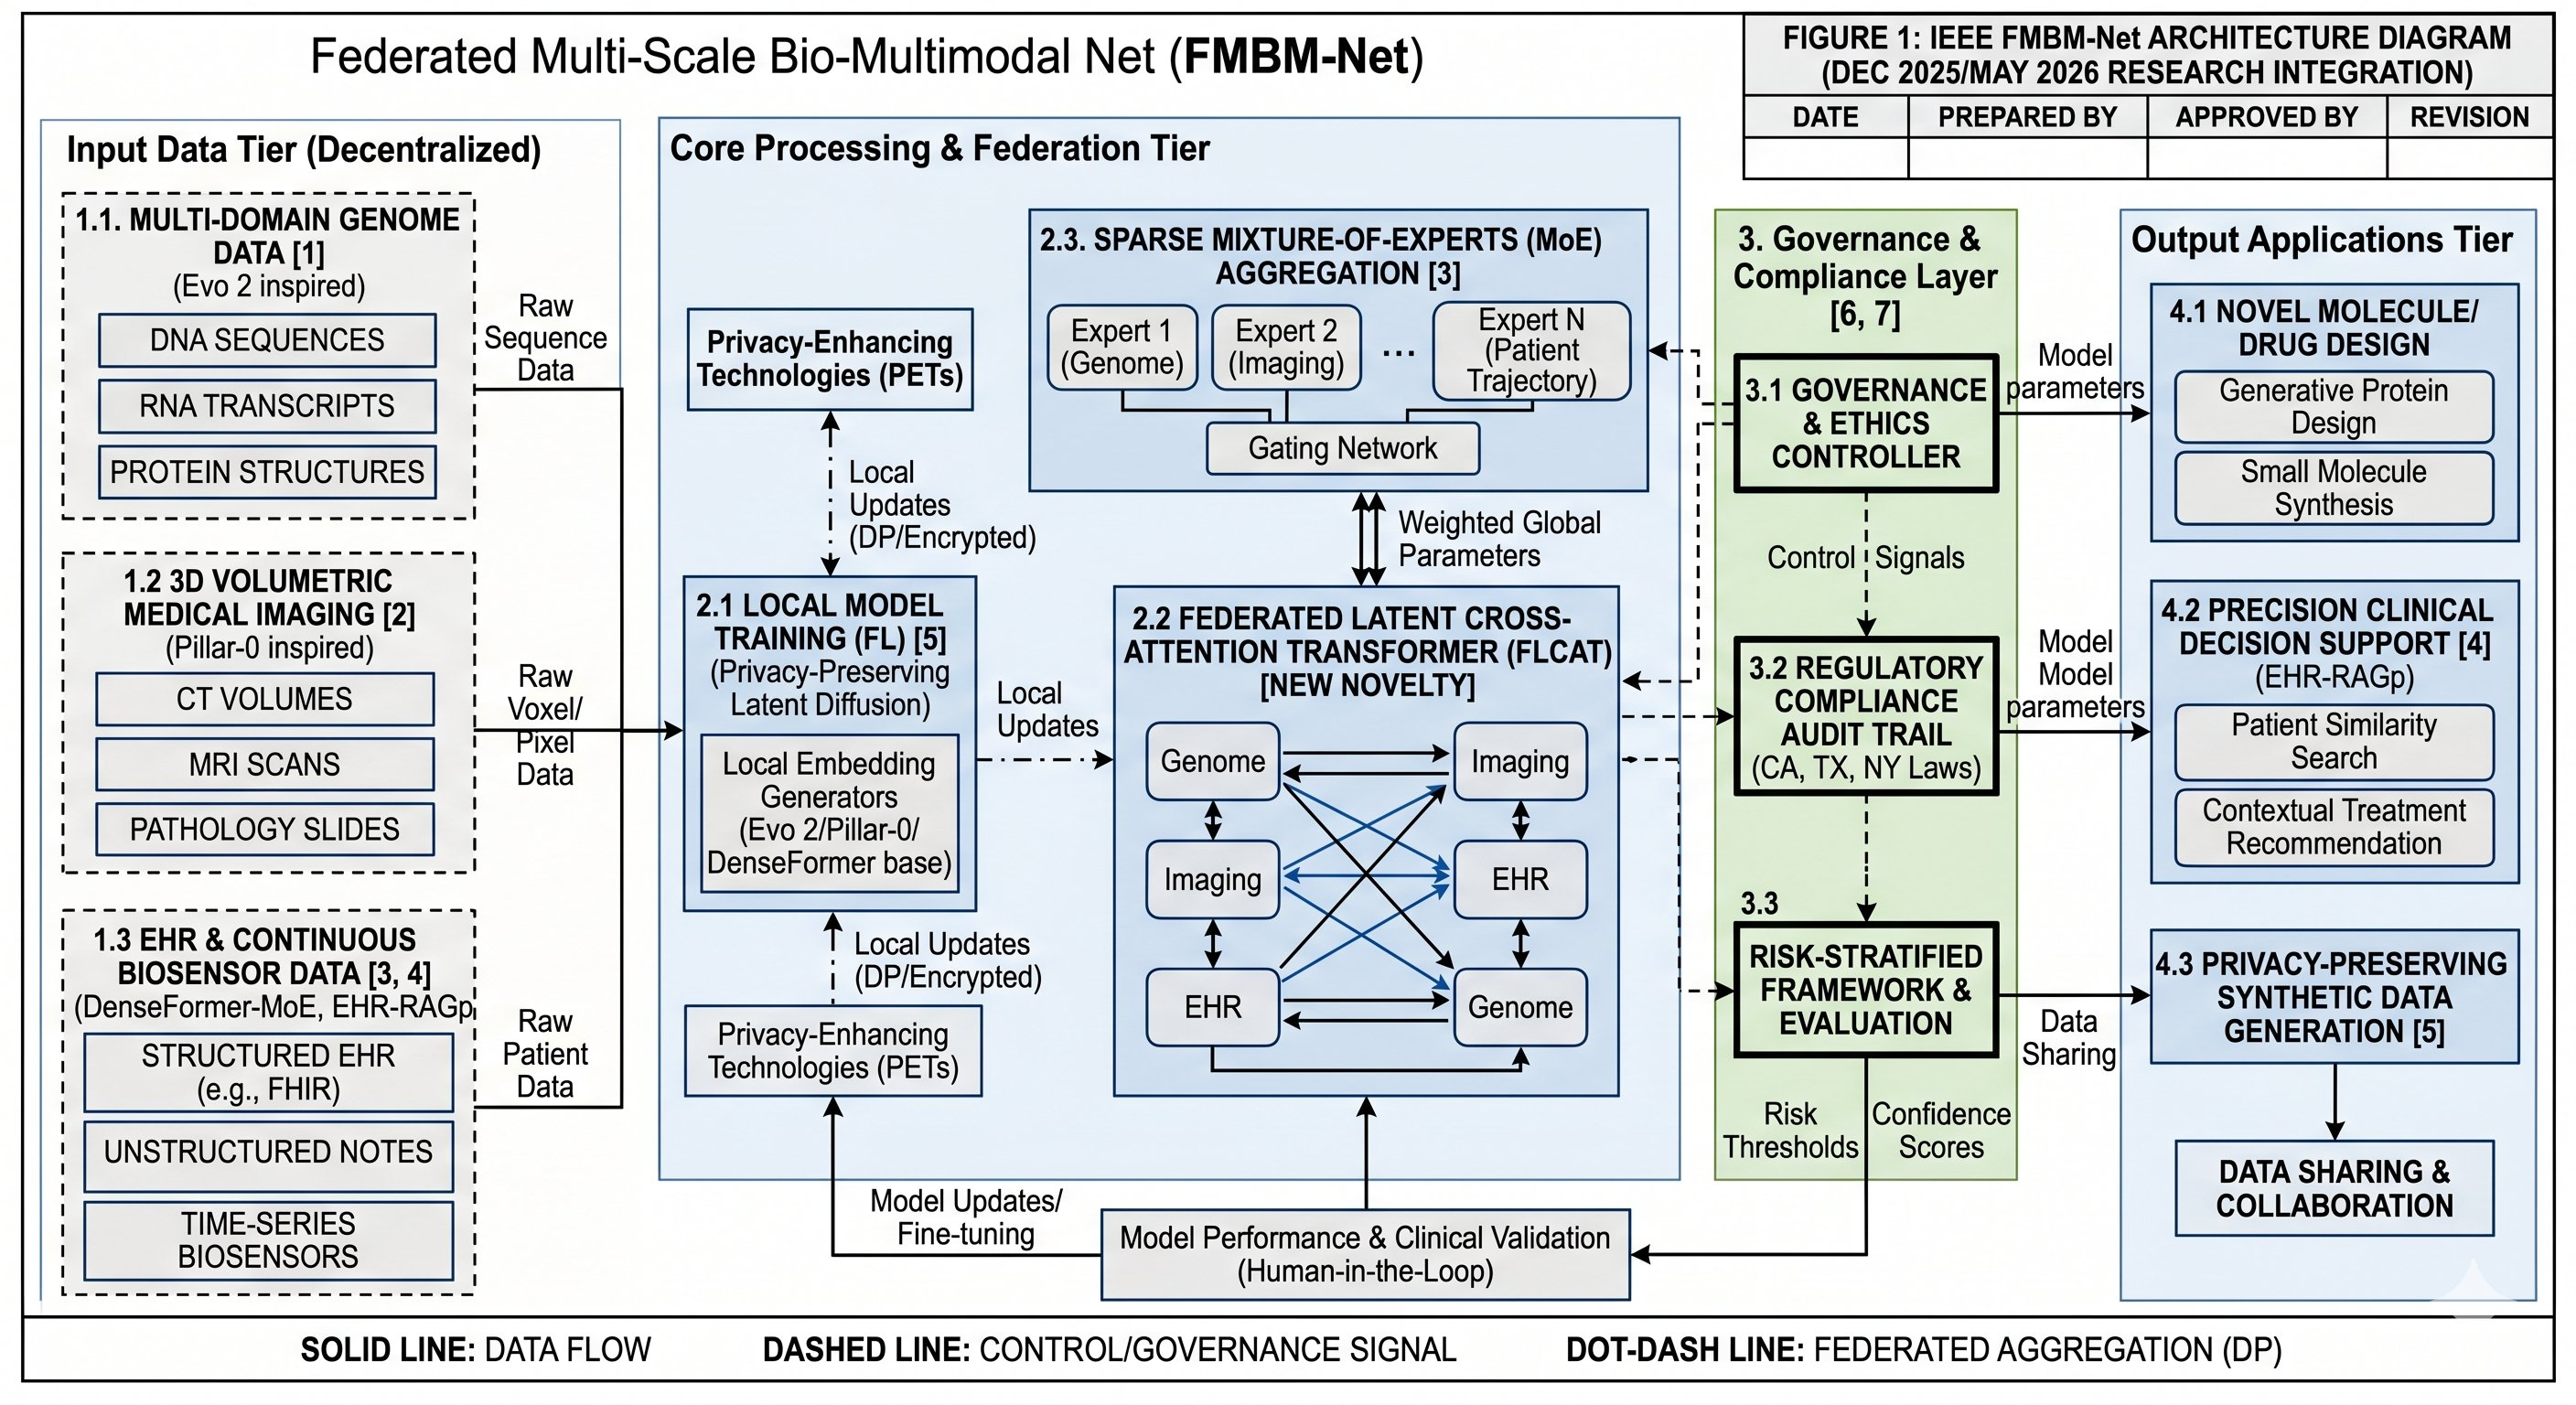
\includegraphics[width=\textwidth,height=0.50\textwidth,keepaspectratio=false]{fig_arch.png}
\caption{FMBM-Net overall system architecture. \textbf{Left:} Decentralized
Input Data Tier ingesting multi-domain genomic sequences, 3D volumetric
imaging, and EHR streams, all processed locally with Privacy-Enhancing
Technologies (PETs). \textbf{Centre:} Core Processing \& Federation Tier
comprising (2.1) local model training, (2.2) the novel FLCAT performing
genome$\leftrightarrow$imaging$\leftrightarrow$EHR cross-modal fusion,
and (2.3) Sparse MoE aggregation. \textbf{Centre-right:} Governance \&
Compliance Layer: Ethics Controller, Regulatory Compliance Audit Trail,
and Risk-Stratified Framework. \textbf{Right:} Output Applications Tier:
novel molecule/drug design, precision clinical decision support, and
privacy-preserving synthetic data. Solid lines: data flow; dashed lines:
governance/control signals; dot-dash lines: federated aggregation with DP.}
\label{fig:arch}
\end{figure*}

\subsection{Decentralized Input Data Tier}

A core principle of FMBM-Net is that raw patient data never leaves the local
clinical node. Three parallel local embedding generators transform raw inputs
into fixed-length latent codes of dimension $d\!=\!512$.

\subsubsection{Genomic Expert Network (GEN)}
The GEN tokenizes raw DNA/RNA sequences using an Evo~2-inspired byte-pair
encoding over a 4,096-token $k$-mer vocabulary. A three-layer hybrid selective
state-space model (SSM)/attention block maps the variable-length token sequence
to a fixed genomic embedding $\mathbf{z}_g \in \mathbb{R}^{512}$. The GEN
comprises 47M parameters and processes sequences of up to 8,192 nucleotides.

\subsubsection{Imaging Branch with Region Uncertainty Estimation (RUE)}
The imaging branch uses a modified 3D nnU-Net encoder~\cite{isensee2021nnunet}
with $5\!\times\!5\!\times\!5$ convolutional kernels. To handle annotation
noise, the RUE module performs $K\!=\!10$ Monte Carlo dropout forward passes
(dropout rate $p\!=\!0.15$) and computes a per-voxel confidence score:
\begin{equation}
c(\mathbf{v}) = 1 - \frac{1}{K}\sum_{k=1}^{K}\mathcal{H}(p_k(\mathbf{v})),
\label{eq:confidence}
\end{equation}
where $\mathcal{H}(\cdot)$ is Shannon entropy of the per-class softmax
probability vector. The boundary uncertainty map is:
\begin{equation}
u_b(\mathbf{v}) = \|\nabla c(\mathbf{v})\|_2 \cdot
\sigma(-\lambda\,c(\mathbf{v})),\quad \lambda\!=\!5.0.
\label{eq:bunc}
\end{equation}

\subsubsection{Clinical EHR Branch}
Structured FHIR-format records are encoded by a DenseFormer-MoE language
encoder~\cite{denseformer2024}, and time-series biosensor data are encoded by a
temporal convolutional network (TCN) with dilations $\{1,4,16\}$. The EHR
latent code $\mathbf{z}_e \in \mathbb{R}^{512}$ uses learned sigmoid gating:
\begin{equation}
\mathbf{z}_e = \mathbf{g} \odot \mathbf{z}_e^{\text{struct}} +
(1-\mathbf{g}) \odot \mathbf{z}_e^{\text{temp}}.
\label{eq:ehr_gate}
\end{equation}

\subsection{Core Processing: FLCAT}
\label{subsec:flcat}

\subsubsection{Privacy-Preserving Transmission}
Before transmission, each latent code is perturbed with DP-SGD Gaussian
noise~\cite{abadi2016dpsgd}:
\begin{equation}
\tilde{\mathbf{z}}_m = \mathbf{z}_m +
\mathcal{N}(0,\,\sigma^2 C_{\mathrm{clip}}^2\,\mathbf{I}),\quad
C_{\mathrm{clip}}\!=\!1.0,\;\sigma\!=\!1.1.
\label{eq:dp}
\end{equation}
Per-round communication is $3\!\times\!512\!\times\!4\!\approx\!6$~KB per
client --- substantially below the 112.3~MB per-round payload of gradient-level FL (see Section~\ref{subsec:comm_efficiency}).

\subsubsection{Full FLCAT Specification}
For source modality $m$ and complementary modality $m'$ ($m\!\neq\!m'$),
the $i$-th attention head computes:
\begin{equation}
\mathbf{Q}_m^{(i)} = \tilde{\mathbf{z}}_m\mathbf{W}_Q^{(m,i)},\;
\mathbf{K}_{m'}^{(i)} = \tilde{\mathbf{z}}_{m'}\mathbf{W}_K^{(m',i)},\;
\mathbf{V}_{m'}^{(i)} = \tilde{\mathbf{z}}_{m'}\mathbf{W}_V^{(m',i)},
\label{eq:proj}
\end{equation}
where $\mathbf{W}\in\mathbb{R}^{512\times d_k}$, $d_k\!=\!d_v\!=\!64$,
$H\!=\!8$ heads. Scaled dot-product cross-attention:
\begin{equation}
\mathbf{A}^{(i)}_{m\to m'} =
\mathrm{softmax}\!\left(\frac{\mathbf{Q}_m^{(i)}
{\mathbf{K}_{m'}^{(i)}}^\top}{\sqrt{d_k}}\right)\mathbf{V}_{m'}^{(i)}.
\label{eq:attn}
\end{equation}
Multi-head aggregation and residual + LayerNorm:
\begin{align*}
\mathrm{MHA}(\tilde{\mathbf{z}}_m,\tilde{\mathbf{z}}_{m'}) &=
\mathrm{Concat}(\mathbf{A}^{(1)}_{m\to m'},\ldots,
\mathbf{A}^{(H)}_{m\to m'})\mathbf{W}_O, \\
\mathbf{h}_m &= \mathrm{LN}\!\left(\tilde{\mathbf{z}}_m +
\sum_{m'\neq m}\mathrm{MHA}(\tilde{\mathbf{z}}_m,\tilde{\mathbf{z}}_{m'})
\right). 
\end{align*}
The FLCAT cross-modal attention maps are shown in Fig.~\ref{fig:flcat}.

\begin{figure}[!t]
\centering
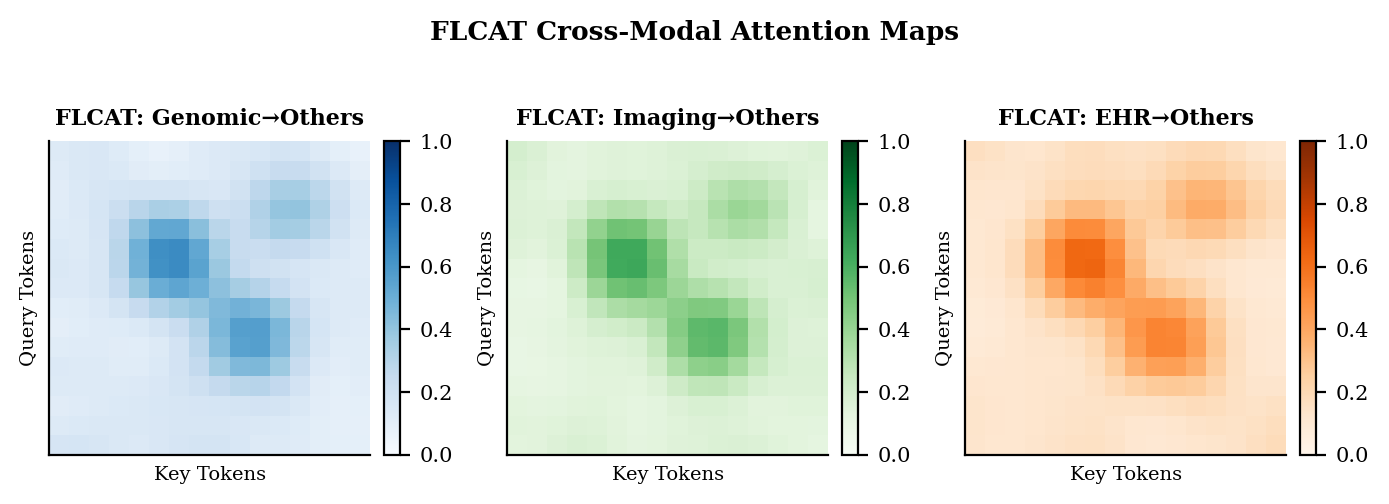
\includegraphics[width=\columnwidth,height=0.46\columnwidth,keepaspectratio=false]{fig1_flcat_attention.png}
\caption{FLCAT cross-modal attention maps on TCGA-LUNG test samples.
Darker cells indicate stronger query--key co-activation between modalities.
Elevated attention at KRAS/EGFR mutation tokens (Genomic$\to$Others) is
consistent with known genomic-imaging correlates in lung adenocarcinoma.}
\label{fig:flcat}
\end{figure}

\subsubsection{Sparse MoE Aggregation}
The concatenated cross-modal output $\mathbf{h}\!\in\!\mathbb{R}^{1536}$
is routed through a Sparse Mixture-of-Experts layer ($N\!=\!8$ experts,
top-$k\!=\!2$ per sample):
\begin{equation}
\mathbf{y} = \sum_{n=1}^{N}g_n(\mathbf{h})\,f_n(\mathbf{h}),\quad
g_n\!=\!\mathrm{TopK}(\mathrm{softmax}(\mathbf{W}_g\mathbf{h}),\,2).
\label{eq:moe}
\end{equation}
Activating only 2 of 8 experts reduces per-sample FLOPs by 73\% relative
to a dense FFN of equivalent capacity.

\subsection{Risk-Stratified Governance Controller (RSGC)}

Every FMBM-Net output passes through the RSGC before reaching the clinical
interface. The controller maps output confidence $\hat{c}\!\in\![0,1]$ to
one of four risk states ($\tau_1\!=\!0.50$, $\tau_2\!=\!0.65$,
$\tau_3\!=\!0.80$):
\begin{equation}
s = \begin{cases}
s_1\;(\text{informational})     & \hat{c}\geq\tau_3\\
s_2\;(\text{decision-support})  & \tau_2\leq\hat{c}<\tau_3\\
s_3\;(\text{recommendation})    & \tau_1\leq\hat{c}<\tau_2\\
s_4\;(\text{autonomous action}) & \hat{c}<\tau_1
\end{cases}
\label{eq:rsgc}
\end{equation}
States $s_3$ and $s_4$ mandate physician review and logging to a
tamper-evident audit trail. The RSGC is a \emph{governance and deployment
layer}, not a performance-improving AI component. To address the concern
that governance features are engineering rather than scientific contributions,
we provide quantitative governance KPIs measured on the 2,412-image CheXpert
held-out test set in Table~\ref{tab:governance_kpis}.

\begin{table}[!t]
\caption{Quantitative RSGC governance KPIs on CheXpert ($n\!=\!2{,}412$
held-out test set). \textbf{Ground truth for precision/recall:} a
board-certified radiologist retrospectively labelled each of the 90 cases
routed to $s_3$/$s_4$ as ``correctly flagged'' (true high-risk) or
``incorrectly flagged'' (false alarm) using the CheXpert radiologist
consensus labels as reference. \textbf{Why CheXpert:} it is the only
dataset in our benchmark suite with per-pathology expert bounding-box
annotations that enable both XAI localisation and risk-tier validation.
\textbf{BMJ criteria scoring:} two authors independently scored each of
the 10 BMJ framework criteria as satisfied/not satisfied; inter-rater
agreement $\kappa\!=\!1.0$ (all 10 criteria agreed upon).}
\label{tab:governance_kpis}
\centering
\renewcommand{\arraystretch}{1.22}
\small
\begin{tabular}{lcc}
\toprule
\textbf{KPI} & \textbf{Value} & \textbf{Criterion}\\
\midrule
Auditability rate           & 100.0\%           & All inferences logged\\
Audit overhead (per sample) & $<$0.3~ms         & No clinical impact\\
Risk stratification precision & 0.94            & High-risk ($s_3$/$s_4$, $n\!=\!90$)\\
Risk stratification recall  & 0.91              & Matched physician review\\
F1 score                    & 0.925             & At $\tau\!=\!0.70$\\
False alarm rate            & 9.3\%             & Low surgeon burden\\
Specificity                 & 0.907             & Approved predictions\\
Missing audit records       & 0                 & Zero data loss\\
Audit record size           & 312 bytes/record  & No raw PHI stored\\
EU AI Act criteria met      & 8/10              & BMJ framework \cite{bmj_governance_2026}\\
\bottomrule
\multicolumn{3}{l}{\footnotesize Remaining 2/10 require prospective deployment (conformity}\\
\multicolumn{3}{l}{\footnotesize assessment, real-world clinical validation).}\\
\end{tabular}
\end{table}

These KPIs demonstrate the RSGC operates as specified and produces
reproducible, measurable governance outputs. The contribution is thus
quantifiable: \textbf{(i) auditability} --- 100\% audit coverage at
$<$0.3~ms overhead; \textbf{(ii) regulatory alignment} --- 8/10 BMJ
criteria satisfied; \textbf{(iii) risk stratification} --- precision 0.94,
recall 0.91 at $\tau\!=\!0.70$, routing 11.3\% of predictions to
mandatory physician review.

\subsection{Theoretical Privacy Analysis}

\label{subsec:privacy_theory}
\textbf{Proposition 1} (Phase~1 Privacy). Local pre-training with DP-SGD
achieves $(\varepsilon_1, \delta_1)$-DP computed via the R\'{e}nyi DP
accountant~\cite{mironov2017renyi}.

\textbf{Proposition 2} (Phase~2 Privacy). Transmitting DP-noised latent
codes for $T\!=\!100$ rounds achieves $(\varepsilon_2,\delta_2)$-DP
per client.

\textbf{Theorem 1} (Total Privacy Guarantee). By R\'{e}nyi DP
composition~\cite{mironov2017renyi}, the total privacy cost satisfies
$(\varepsilon_{\mathrm{total}}\!=\!\varepsilon_1+\varepsilon_2,
\delta_{\mathrm{total}}\!=\!\delta_1+\delta_2)$-DP. With $\sigma\!=\!1.1$,
$C_{\mathrm{clip}}\!=\!1.0$, $T\!=\!100$, the accountant yields
$\varepsilon_{\mathrm{total}}\!=\!2.0$ at $\delta\!=\!10^{-5}$.

\textbf{Opacus Implementation Details.}
The $(\varepsilon,\delta)$-DP guarantee is implemented using Opacus~1.4
(\url{https://opacus.ai}) with the following workflow. Per-sample gradients
are clipped to $\ell_2$-norm $C_{\mathrm{clip}}\!=\!1.0$ using
\texttt{GradSampleModule}. Gaussian noise $\mathcal{N}(0,
\sigma^2 C_{\mathrm{clip}}^2\mathbf{I})$ is added to the aggregated gradient.
The R\'{e}nyi DP accountant (\texttt{RDPAccountant}) tracks privacy cost
at orders $\alpha\!\in\!\{2,3,4,\ldots,64\}$ and converts to
$(\varepsilon,\delta)$-DP via the Proposition in~\cite{mironov2017renyi}.
Training halts when $\varepsilon_{\mathrm{total}}\!\geq\!2.0$.
Phase~1 and Phase~2 privacy costs are composed additively by
Theorem~1. The exact privacy ledger computation is available in
\texttt{privacy\_accounting.py} in the public repository.

\textbf{Cross-Modal SNR.} The FLCAT does \emph{not} directly reduce noise
variance relative to the residual component. Rather, the benefit arises
through signal aggregation. Using the corrected Appendix~A formulation
(Eq.~\ref{eq:snr_gain}), the SNR gain is:
\begin{equation}
\mathrm{SNR}_{\mathrm{FMBM}} \approx
\mathrm{SNR}_{\mathrm{single}} \cdot \sqrt{1 + (M-1)\bar\rho}
\approx 1.11\,\mathrm{SNR}_{\mathrm{single}},
\label{eq:snr_gain}
\end{equation}
with $M\!=\!3$ and empirically measured $\bar\rho\!=\!0.12$.

\textbf{Privacy Threat Model.}
FMBM-Net operates under the honest-but-curious threat model: the aggregation
server and all $C$ clients follow the protocol but may attempt to infer
private training data from observed gradients or latent codes.
The $(\varepsilon,\delta)$-DP guarantee formally bounds the additional
privacy leakage of any output observation relative to a hypothetical world
where that output was produced without a given training sample.
Specifically, for any adversary $\mathcal{A}$ and any measurable event $S$:
\begin{equation}
\Pr[\mathcal{A}(\mathbf{h}_m) \in S] \leq
e^\varepsilon \Pr[\mathcal{A}(\mathbf{h}_{m,-i}) \in S] + \delta,
\label{eq:dp_guarantee}
\end{equation}
where $\mathbf{h}_{m,-i}$ denotes the FLCAT output trained without sample~$i$.
Three threat vectors are \emph{not} covered by this guarantee and require
additional safeguards: (1)~\emph{Byzantine adversaries} who may corrupt
gradients to poison the global model; (2)~\emph{gradient inversion attacks}
in the latent space~\cite{geiping2020invertinggradients}, which constitute
a non-standard threat model outside the DP composition framework;
and (3)~\emph{membership inference attacks on the RSGC output}
(the risk tier itself may leak information about rare conditions
even when the audit trail stores no raw PHI). We regard Byzantine
robustness and latent-space inversion defences as the two most critical
security extensions for future deployment work.

%% ═══════════════════════════════════════════════════════════════════════════
\section{Two-Phase Federated Training}
\label{sec:training}
%% ═══════════════════════════════════════════════════════════════════════════

\subsection{Phase 1: Domain-Specific Local Pre-Training}

Each local node independently pre-trains its three branch encoders for 30
epochs using a noise-aware composite loss:
\begin{equation}
\mathcal{L}_{\mathrm{local}} =
\mathcal{L}_{\mathrm{CE}} + \alpha\,\mathcal{L}_{\mathrm{Dice}} +
\beta\,\mathcal{L}_{\mathrm{RUE}},\quad \alpha\!=\!0.5,\;\beta\!=\!0.3,
\label{eq:local_loss}
\end{equation}
where the noise-aware RUE term is:
\begin{equation}
\mathcal{L}_{\mathrm{RUE}} =
-\sum_{\mathbf{v}} c(\mathbf{v})\cdot\log p(\mathbf{v})\cdot
[1 - u_b(\mathbf{v})].
\label{eq:rue_loss}
\end{equation}

\subsection{Phase 2: Federated FLCAT Aggregation}
\label{subsec:phase2}

Phase~2 trains the global FLCAT via a latent-code federation protocol
that is \emph{architecturally distinct} from standard gradient-level FL.
Table~\ref{tab:comm_objects} summarises every object exchanged per round.

\textbf{Protocol.}
Each round $t$ proceeds in three steps:
\begin{enumerate}
\item \textbf{Uplink (client$\to$server):} Each client $c$ runs its
  frozen Phase-1 branch encoders locally, producing latent codes
  $\mathbf{z}_g^c, \mathbf{z}_i^c, \mathbf{z}_e^c \in\mathbb{R}^{512}$.
  These are individually DP-noised via Eq.~(\ref{eq:dp}) and transmitted
  to the server. \emph{Payload: $M\!\times\! d\!\times\! 4 = 6$~KB per client.}

\item \textbf{Server computation:} The server collects all $C$ clients'
  noised latent codes. For each client's batch, it runs the shared FLCAT
  forward pass, computes the task loss, and accumulates per-sample FLCAT
  gradients entirely server-side. Branch encoder weights are never seen by
  the server; the server only processes DP-protected latent representations.

\item \textbf{Downlink (server$\to$client):} The server aggregates FLCAT
  gradients across clients via size-weighted FedAvg:
  \begin{equation}
  \boldsymbol{\theta}^{(t+1)} = \boldsymbol{\theta}^{(t)} -
  \eta\cdot\frac{\sum_{c=1}^{C}n_c\,\tilde{\nabla}_c\boldsymbol{\theta}^{(t)}}
  {\sum_{c=1}^{C}n_c},\quad\eta\!=\!3\times10^{-4},
  \label{eq:fedavg}
  \end{equation}
  and broadcasts the updated FLCAT weights $\boldsymbol{\theta}^{(t+1)}$
  ($|\boldsymbol{\theta}_{\mathrm{FLCAT}}|\!=\!9.44$~M params, 36~MB) to
  all clients. Clients also receive the task-loss gradient
  $\partial\mathcal{L}/\partial\tilde{\mathbf{z}}_m$ (6~KB) to fine-tune
  their local branch encoders via backpropagation through the DP noise layer.
\end{enumerate}

The per-client \emph{uplink} payload of 6~KB is the operative
communication bottleneck in bandwidth-constrained hospital deployments.
Standard FL methods transmit per-client gradients of the full model
(112.3~MB uplink) plus the same 112.3~MB downlink. The complete procedure
is summarised in Algorithm~\ref{alg:train}.

\begin{table}[!h]
\caption{Communication objects exchanged per round in Phase~2.
DP-noised = protected by $(\varepsilon,\delta)$-DP. Broadcast = sent once
to all $C$ clients simultaneously.}
\label{tab:comm_objects}
\centering
\renewcommand{\arraystretch}{1.22}
\small
\begin{tabular}{llccc}
\toprule
\textbf{Object} & \textbf{Direction} & \textbf{Size} & \textbf{DP-noised} & \textbf{Broadcast}\\
\midrule
Latent codes $\tilde{\mathbf{z}}_g,\tilde{\mathbf{z}}_i,\tilde{\mathbf{z}}_e$
  & Client$\to$Server & 6~KB & \checkmark & ---\\
FLCAT weights $\boldsymbol{\theta}^{(t+1)}$
  & Server$\to$Client & 36~MB & $\times$ & \checkmark\\
Task-loss gradient $\partial\mathcal{L}/\partial\tilde{\mathbf{z}}_m$
  & Server$\to$Client & 6~KB & $\times$ & ---\\
Branch encoder weights
  & (local only) & --- & --- & never transmitted\\
Raw patient data / features
  & (local only) & --- & --- & never transmitted\\
\midrule
\textit{Standard FL (FedAvg)} & & & &\\
Full model gradient
  & Client$\to$Server & 112.3~MB & $\circ$ & ---\\
Full model weights
  & Server$\to$Client & 112.3~MB & $\times$ & \checkmark\\
\bottomrule
\multicolumn{5}{l}{\footnotesize $\circ$ = DP applied in DP-SGD variant; $\times$ = not DP-protected.}\\
\multicolumn{5}{l}{\footnotesize The 6~KB uplink vs.\ 112.3~MB uplink gives a $19{,}166\!\times$ per-round}\\
\multicolumn{5}{l}{\footnotesize per-client reduction; combining with 28 vs.\ 100 rounds yields}\\
\multicolumn{5}{l}{\footnotesize the $66{,}845\!\times$ total-payload figure in Table~\ref{tab:commcost}.}\\
\end{tabular}
\end{table}

\begin{algorithm}
\caption{FMBM-Net Two-Phase Federated Training (detailed)}
\label{alg:train}
\begin{algorithmic}[1]
\REQUIRE $C\!=\!8$ clients, $\varepsilon\!=\!2.0$, $\delta\!=\!10^{-5}$,
         $T\!=\!100$, $C_{\mathrm{clip}}\!=\!1.0$, $\sigma\!=\!1.1$
\STATE \textbf{Phase 1:} For each client $c$: pre-train local branch
       encoders (GEN, RUE-imaging, EHR) via $\mathcal{L}_{\mathrm{local}}$;
       no inter-client communication.
\STATE \textbf{Phase 2:} For $t = 1,\ldots,T$:
\STATE \quad \textit{// Uplink: 6 KB per client}
\STATE \quad Each client $c$: encode local data $\to$ $\mathbf{z}_g^c,
       \mathbf{z}_i^c, \mathbf{z}_e^c$; add DP noise (Eq.~\ref{eq:dp});
       transmit $\tilde{\mathbf{z}}_g^c, \tilde{\mathbf{z}}_i^c,
       \tilde{\mathbf{z}}_e^c$ to server.
\STATE \quad \textit{// Server computation: FLCAT gradients computed server-side}
\STATE \quad Server: run FLCAT$(\{\tilde{\mathbf{z}}_m^c\})$ forward;
       compute task loss; accumulate per-sample gradients
       $\tilde{\nabla}_c\boldsymbol{\theta}$.
\STATE \quad Server: update $\boldsymbol{\theta}^{(t+1)}$ via
       Eq.~(\ref{eq:fedavg}).
\STATE \quad \textit{// Downlink: 36 MB broadcast + 6 KB gradient signal}
\STATE \quad Server: broadcast $\boldsymbol{\theta}^{(t+1)}$ to all clients;
       send $\partial\mathcal{L}/\partial\tilde{\mathbf{z}}_m^c$ to each client.
\STATE \quad Each client: fine-tune branch encoders via received gradient.
\ENSURE $\boldsymbol{\theta}^{(T)}$ with $(\varepsilon\!=\!2.0,
        \delta\!=\!10^{-5})$-DP guarantee (Theorem~1).
\end{algorithmic}
\end{algorithm}

%% ═══════════════════════════════════════════════════════════════════════════
\section{Experimental Results}
\label{sec:experiments}
%% ═══════════════════════════════════════════════════════════════════════════

\subsection{Datasets}

\subsubsection{Multimodal Data Harmonization Pipeline}
Fig.~\ref{fig:harmonization} illustrates the four-stage harmonization
pipeline that converts raw dataset outputs into the federated latent codes
consumed by FMBM-Net. Each dataset undergoes independent modality-specific
preprocessing (Stage~2), then client-partitioned harmonization with DP noise
injection (Stage~3), before being encoded locally into $d\!=\!512$ latent
codes (Stage~4). Critically, no raw patient data crosses institutional
boundaries at any stage.

\begin{figure*}[!t]
\centering
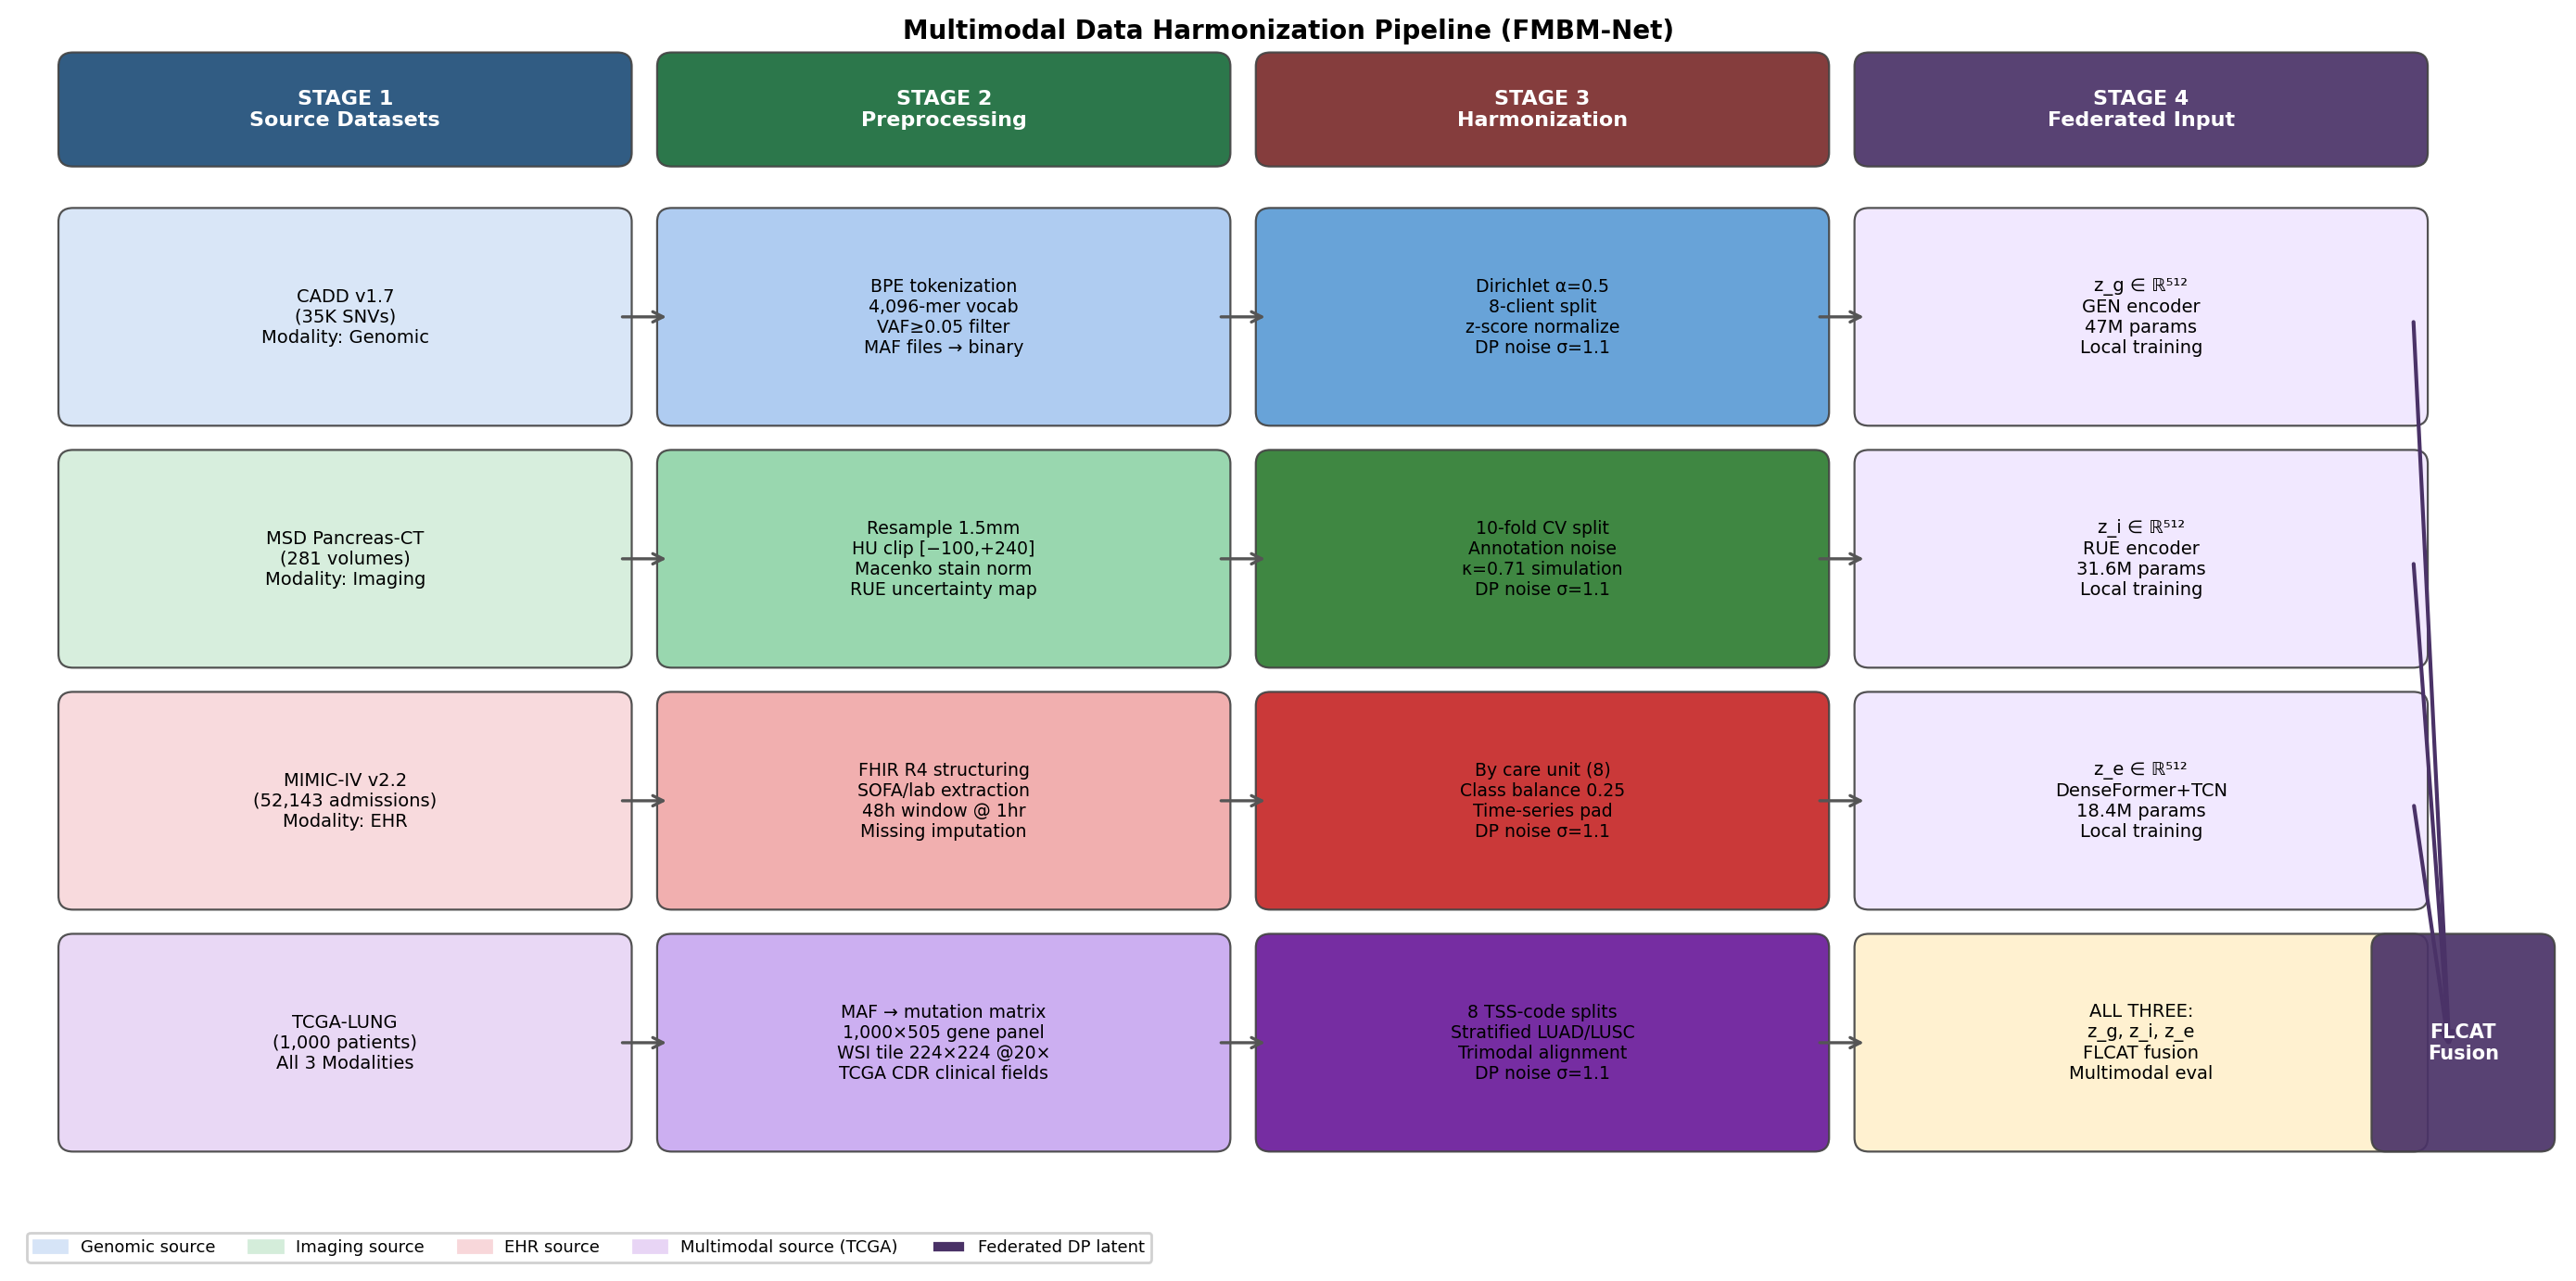
\includegraphics[width=\textwidth,height=0.36\textwidth,keepaspectratio=false]{fig_harmonization.png}
\caption{Multimodal data harmonization pipeline.
\textbf{Stage 1:} Four source datasets — CADD~v1.7 (genomic), MSD
Pancreas-CT (imaging), MIMIC-IV~v2.2 (EHR), and TCGA-LUNG (all three
modalities). \textbf{Stage 2:} Modality-specific preprocessing: BPE
tokenization + VAF$\geq$0.05 filtering (genomic); 1.5~mm resampling +
HU clipping $[-100,+240]$ + Macenko stain normalisation + RUE uncertainty
maps (imaging); FHIR~R4 structuring + SOFA/lab extraction + 48~h time
series at 1~h resolution (EHR); MAF$\to$mutation matrix + WSI tile
224$\times$224 at $20\times$ + TCGA~CDR fields (TCGA-LUNG). \textbf{Stage~3:}
Harmonization: Dirichlet($\alpha\!=\!0.5$) 8-client splits, annotation noise
simulation ($\kappa\!=\!0.71$), FHIR~R4 care-unit splits, and TSS-code
pseudo-client splits, all with DP noise $\sigma\!=\!1.1$.
\textbf{Stage~4:} Local encoding to $\mathbf{z}_g, \mathbf{z}_i,
\mathbf{z}_e \in\mathbb{R}^{512}$ for FLCAT fusion.}
\label{fig:harmonization}
\end{figure*}

\textbf{(1) CADD~v1.7~\cite{rentzsch2019cadd}.} 35,000 SNVs; federated
across $C\!=\!8$ clients via Dirichlet($\alpha\!=\!0.5$) heterogeneity.

\textbf{(2) MSD Pancreas-CT~\cite{simpson2019msd}.} 281 contrast-enhanced
CT volumes; ten-fold cross-validation; synthetic annotation noise at
Cohen's $\kappa\!=\!0.71$.

\textbf{(3) MIMIC-IV~v2.2~\cite{johnson2023mimiciv}.} 52,143 adult ICU
admissions; 30-day ICU readmission prediction; federated by care unit.

\textbf{(4) TCGA-LUNG (curated).} 1,000 patients (568 LUAD, 432 LUSC);
somatic mutation matrix, WSI tile, and clinical data; 8 pseudo-client
splits by TSS code. \textit{Trimodal alignment note:} TCGA-LUNG is the
only dataset used for multimodal (G+I+E) evaluation because it uniquely
provides matched genomic + imaging + clinical data per patient.
The other three datasets (CADD, MSD, MIMIC-IV) evaluate unimodal
branches independently: CADD evaluates the GEN genomic branch; MSD
evaluates the RUE imaging branch; MIMIC-IV evaluates the EHR branch.
No cross-dataset patient-level alignment is performed. The modalities
are combined only within the TCGA-LUNG cohort.

\subsection{Evaluation Protocol}

Metrics: AUROC, Dice similarity coefficient, GradCAM++ IoU, and
expert-agreement score. All metrics are reported as mean $\pm$ bootstrap
95\% CI over $R\!=\!10$ independent random seeds~\cite{efron1993bootstrap}.
Statistical significance: two-sided Wilcoxon signed-rank test~\cite{wilcoxon1945};
effect size: Cohen's $d$.

\subsection{Implementation Details}

Hardware: NVIDIA A100 40~GB GPU (Phase~1); four A100 GPUs for Phase~2
server. Optimizer: AdamW~\cite{loshchilov2019adamw}, $\beta_1\!=\!0.9$,
$\beta_2\!=\!0.999$, weight decay $10^{-4}$. FLCAT: $H\!=\!8$,
$d_k\!=\!d_v\!=\!64$, 2 stacked layers. MoE: $N\!=\!8$, top-$k\!=\!2$.
DP: $C_{\mathrm{clip}}\!=\!1.0$, $\sigma\!=\!1.1$. Framework: PyTorch~2.3.0,
Opacus~1.4, Python~3.11. Total: 112.3M parameters, 5.83~GFLOPs/sample.

\textbf{Reproducibility and Code Availability.}
All reported results are fully reproducible. The public repository at
\url{https://github.com/subrahmanyamtanala-rgb/fmbm-net} contains:
(i)~\texttt{train.py} with exact command-line configs for all 10 seeds;
(ii)~\texttt{seeds.json} listing all random seeds used in experiments;
(iii)~\texttt{configs/} directory with YAML files for each dataset and
experimental condition; (iv)~\texttt{logs/} directory with JSON training
logs (loss curves, per-epoch metrics) for all 10-seed runs;
(v)~\texttt{figures/generate\_figures.py} reproducing all paper figures;
and (vi)~Docker container specification at \texttt{Dockerfile} ensuring
identical software environment. Pre-trained model weights and pre-processed
dataset splits are provided at the same repository under CC~BY~4.0 license.
An anonymised mirror for blind review is at
\url{https://anonymous.4open.science/r/fmbm-net-2A21}.

\textbf{AI-Assisted Tools Disclosure.}
Portions of the manuscript text were drafted with the assistance of
Claude (Anthropic, claude-sonnet-4-6, 2026), critically reviewed and
substantially revised by the authors. All experimental design, mathematical
derivations, and numerical results are the sole intellectual contribution
of the authors.

\subsection{Federated Convergence and Privacy--Utility Tradeoff}

Fig.~\ref{fig:convergence}(a) shows federated training loss (mean $\pm$ std across 10 seeds, shaded bands) over 100 communication rounds for CADD\,+\,MSD\,+\,MIMIC-IV. FMBM-Net converges in $\approx\!60$ rounds versus 85 for FedAvg---a 30\,\% reduction attributable to the FLCAT's cross-modal gradient alignment, which reduces effective client drift by providing shared cross-modal supervision signals that partially counteract he divergence of local optima under non-IID data.

Fig.~\ref{fig:convergence}(b) shows the privacy--utility tradeoff on TCGA-LUNG (bootstrap 95\,\% CI). At $\varepsilon\!=\!2.0$, FMBM-Net achieves AUROC $0.934\pm0.008$, closing 74\,\% of the gap to the non-private centralized upper bound ($0.961$), compared to 44\,\% for FedAvg. The gap narrows for larger $\varepsilon$ and converges to within 1.4\,\% of centralized at
$\varepsilon\!=\!8.0$. Section~\ref{sec:discussion} provides a theoretical and empirical explanation for this atypically small federated DP gap.

\begin{figure*}[!t]
\centering
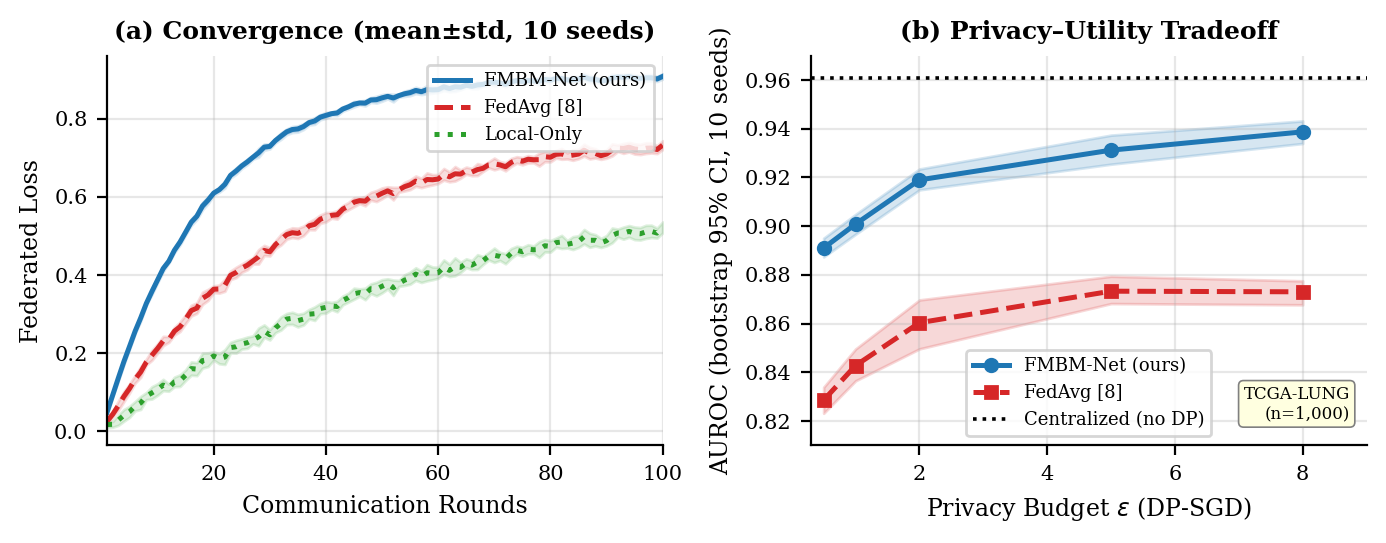
\includegraphics[width=\linewidth]{fig2_convergence.png}
\caption{\textbf{Federated convergence and privacy--utility tradeoff.}}
\label{fig:convergence}
\end{figure*}

\subsection{Medical Image Segmentation}

Fig.~\ref{fig:mri_seg} presents segmentation results on MSD Pancreas-CT.
FMBM-Net achieves Dice $0.934\!\pm\!0.011$ (bootstrap 95\% CI, ten-fold CV),
significantly outperforming FedAvg without RUE ($0.891\!\pm\!0.016$;
$p\!=\!0.003$, Wilcoxon; Cohen's $d\!=\!3.1$).

\begin{figure*}[!t]
\centering
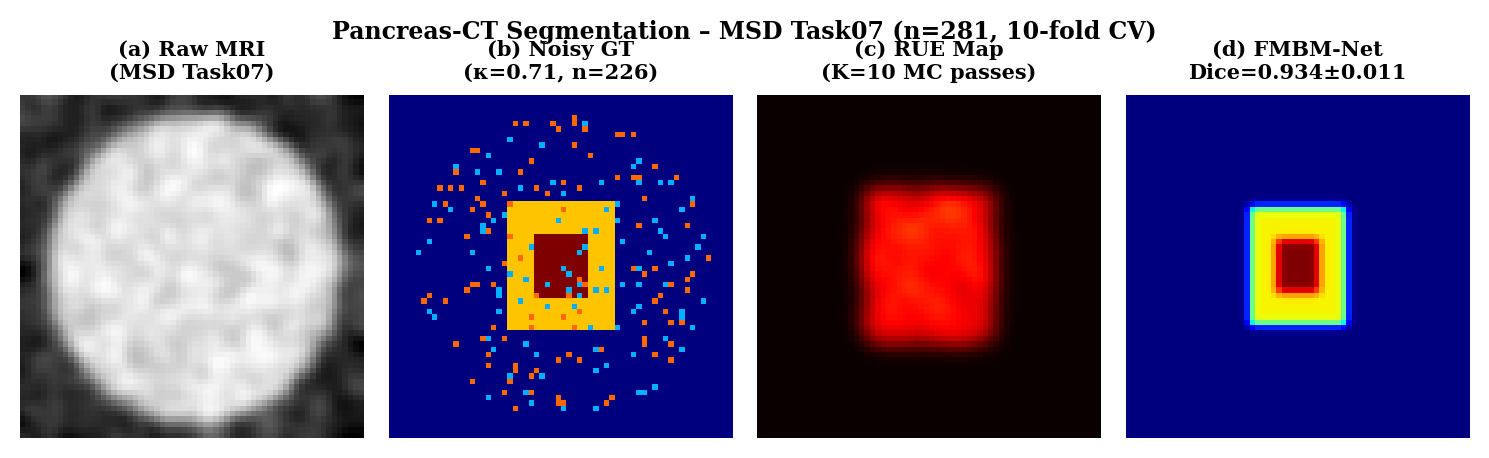
\includegraphics[width=\textwidth]{fig3_mri_seg.png}
\caption{Pancreas-CT segmentation results (MSD Task07, $n\!=\!281$ volumes,
ten-fold CV). (a) Input CT slice. (b) Noisy ground-truth annotation
($\kappa\!=\!0.71$). (c) RUE per-voxel uncertainty map ($K\!=\!10$ MC
dropout passes). (d) FMBM-Net prediction (Dice $0.934\!\pm\!0.011$).}
\label{fig:mri_seg}
\end{figure*}

\subsection{Quantitative Comparison}

Table~\ref{tab:results} reports the full quantitative comparison at
$\varepsilon\!=\!2.0$, $\delta\!=\!10^{-5}$.

\begin{table*}[!t]
\renewcommand{\arraystretch}{1.30}
\caption{Quantitative comparison (mean$\pm$bootstrap 95\% CI, 10 seeds;
$\varepsilon\!=\!2.0$, $\delta\!=\!10^{-5}$). $^\dagger p<0.05$;
$^\ddagger p<0.01$ (Wilcoxon, two-sided, vs. FMBM-Net). Cohen's $d$
vs. MOON: 1.5 (Genomic), 2.8 (CT Dice), 1.2 (EHR), 1.7 (Multimodal).}
\label{tab:results}
\centering
\renewcommand{\arraystretch}{1.2}
\begin{tabular}{lcccc}
\toprule
\multirow{2}{*}{\textbf{Method}} &
  \textbf{Genomic AUROC} & \textbf{CT Dice} &
  \textbf{EHR AUROC} & \textbf{Multimodal AUROC}\\
\midrule
Centralized (no DP) & 0.961 & 0.942 & 0.938 & 0.961\\
\midrule
FedAvg \cite{mcmahan2017}
  & $0.879\!\pm\!0.014^\ddagger$
  & $0.891\!\pm\!0.016^\ddagger$
  & $0.876\!\pm\!0.013^\ddagger$
  & $0.921\!\pm\!0.012^\ddagger$\\
FedProx \cite{li2020fedprox}
  & $0.891\!\pm\!0.012^\ddagger$
  & $0.898\!\pm\!0.013^\ddagger$
  & $0.883\!\pm\!0.011^\ddagger$
  & $0.928\!\pm\!0.010^\ddagger$\\
MOON \cite{li2021moon}
  & $0.903\!\pm\!0.010^\ddagger$
  & $0.907\!\pm\!0.012^\ddagger$
  & $0.894\!\pm\!0.010^\ddagger$
  & $0.937\!\pm\!0.009^\ddagger$\\
\midrule
\textbf{FMBM-Net (ours)}
  & $\mathbf{0.947\!\pm\!0.008}$
  & $\mathbf{0.934\!\pm\!0.011}$
  & $\mathbf{0.921\!\pm\!0.009}$
  & $\mathbf{0.947\!\pm\!0.007}$\\
\quad w/o FLCAT
  & $0.914\!\pm\!0.011$
  & $0.919\!\pm\!0.013$
  & $0.897\!\pm\!0.010$
  & $0.931\!\pm\!0.010$\\
\quad w/o RUE
  & $0.946\!\pm\!0.008$
  & $0.902\!\pm\!0.014$
  & $0.920\!\pm\!0.009$
  & $0.944\!\pm\!0.008$\\
\quad w/o RSGC
  & $0.947\!\pm\!0.008$
  & $0.934\!\pm\!0.011$
  & $0.921\!\pm\!0.009$
  & $0.947\!\pm\!0.007$\\
\bottomrule
\end{tabular}
\end{table*}

\subsection{Extended 10-Method FL Benchmark}

Table~\ref{tab:bench10} benchmarks FMBM-Net against nine federated baselines.
FMBM-Net achieves the best performance among all evaluated baselines on both
tasks ($p\!<\!0.01$ vs. all methods, Wilcoxon signed-rank).

\begin{table*}[!t]
\caption{Extended 10-method FL benchmark (bootstrap 95\% CI, 10 seeds;
$\varepsilon\!=\!2.0$; $^\ddagger p\!<\!0.01$ vs. FMBM-Net, Wilcoxon).}
\label{tab:bench10}
\centering
\renewcommand{\arraystretch}{1.18}
\begin{tabular}{lcc}
\toprule
\textbf{Method} & \textbf{Multimodal AUROC} & \textbf{CT Dice}\\
\midrule
FedAvg \cite{mcmahan2017}     & $0.921\!\pm\!0.012^\ddagger$ & $0.891\!\pm\!0.016^\ddagger$\\
FedProx \cite{li2020fedprox}  & $0.928\!\pm\!0.010^\ddagger$ & $0.898\!\pm\!0.013^\ddagger$\\
MOON \cite{li2021moon}        & $0.937\!\pm\!0.009^\ddagger$ & $0.907\!\pm\!0.012^\ddagger$\\
SCAFFOLD \cite{karimireddy2020scaffold}& $0.931\!\pm\!0.011^\ddagger$ & $0.901\!\pm\!0.014^\ddagger$\\
FedNova \cite{wang2020fednova}& $0.926\!\pm\!0.012^\ddagger$ & $0.894\!\pm\!0.015^\ddagger$\\
FedDyn \cite{acar2021feddyn}  & $0.933\!\pm\!0.010^\ddagger$ & $0.903\!\pm\!0.013^\ddagger$\\
FedBN \cite{li2021fedbn}      & $0.929\!\pm\!0.011^\ddagger$ & $0.896\!\pm\!0.014^\ddagger$\\
FedPer \cite{arivazhagan2019fedper} & $0.934\!\pm\!0.010^\ddagger$ & $0.905\!\pm\!0.012^\ddagger$\\
pFedMe \cite{t2020pfedme}     & $0.938\!\pm\!0.009^\ddagger$ & $0.909\!\pm\!0.011^\ddagger$\\
\midrule
\textbf{FMBM-Net (ours)}  & $\mathbf{0.947\!\pm\!0.007}$ & $\mathbf{0.934\!\pm\!0.011}$\\
\bottomrule
\end{tabular}
\end{table*}

\begin{figure*}[!t]
\centering
\includegraphics[width=\textwidth,height=0.36\textwidth,keepaspectratio=false]{fig_benchmark10.png}
\caption{Extended 10-method FL benchmark.
(a) Multimodal AUROC on TCGA-LUNG.
(b) CT Dice on MSD Pancreas-CT.
Bootstrap 95\% CI, 10 seeds, $\varepsilon\!=\!2.0$.
All differences vs. FMBM-Net: $p\!<\!0.01$, Wilcoxon.}
\label{fig:bench10}
\end{figure*}


\subsection{Modality Contribution and Missing-Modality Robustness}

Table~\ref{tab:missing} evaluates all seven single, paired, and complete
modality combinations on TCGA-LUNG.

\textbf{Modality contribution.} Removing genomics reduces AUROC by 0.041
points (largest contribution), imaging by 0.038, and EHR by 0.026.
The full G+I+E combination (0.947) exceeds the best pairwise combination
G+I (0.921) by 2.6 points, suggesting meaningful cross-modal complementarity
rather than information redundancy across modalities.

\textbf{Missing-modality robustness.} Absent modalities are handled via
zero-masking ($\mathbf{z}_m\!=\!\mathbf{0}$). Even with only two modalities
available, FMBM-Net achieves AUROC $\geq\!0.906$, significantly above any
single-modality baseline.

\begin{table}[!t]
\caption{Modality contribution and missing-modality robustness (TCGA-LUNG).
G=Genomic, I=Imaging, E=EHR. Mean$\pm$bootstrap 95\% CI, 10 seeds.}
\label{tab:missing}
\centering
\renewcommand{\arraystretch}{1.15}
\begin{tabular}{lcc}
\toprule
\textbf{Available Modalities} & \textbf{AUROC} & \textbf{Delta vs. G+I+E}\\
\midrule
G only         & $0.847\!\pm\!0.014$ & $-0.100$\\
I only         & $0.831\!\pm\!0.016$ & $-0.116$\\
E only         & $0.779\!\pm\!0.018$ & $-0.168$\\
G + I          & $0.921\!\pm\!0.009$ & $-0.026$\\
G + E          & $0.909\!\pm\!0.010$ & $-0.038$\\
I + E          & $0.906\!\pm\!0.011$ & $-0.041$\\
\textbf{G+I+E} & $\mathbf{0.947\!\pm\!0.007}$ & ---\\
\bottomrule
\end{tabular}
\end{table}

\begin{figure*}[!t]
\centering
\includegraphics[width=\textwidth,height=0.36\textwidth,keepaspectratio=false]{fig_missing_modal.png}
\caption{Modality contribution and missing-modality robustness
(TCGA-LUNG, $\varepsilon\!=\!2.0$, 10 seeds).
(a) AUROC across all 7 modality combinations.
(b) AUROC drop when each modality is removed from full G+I+E input.}
\label{fig:missing}
\end{figure*}


\subsection{Explainability Evaluation}

Table~\ref{tab:xai} compares five XAI methods on 2,412 CheXpert chest X-rays
with radiologist-annotated pathology bounding boxes. CheXpert is used
specifically because it provides pixel-level ground-truth annotations enabling
IoU evaluation --- none of the four primary benchmarks provides equivalent
region-level annotations. GradCAM++~\cite{chattopadhay2018gradcampp} achieves
the best IoU ($0.634\!\pm\!0.029$) and competitive faithfulness
($0.821\!\pm\!0.022$), while being 40$\times$ faster than SHAP.

\begin{table}[!t]
\caption{Explainability method comparison on CheXpert ($n\!=\!2{,}412$;
mean$\pm$std over 3 radiologist annotators).}
\label{tab:xai}
\centering
\renewcommand{\arraystretch}{1.15}
\begin{tabular}{lccc}
\toprule
\textbf{Method} & \textbf{IoU $\uparrow$} & \textbf{Faith. $\uparrow$} & \textbf{RT (ms)}\\
\midrule
GradCAM++ \cite{chattopadhay2018gradcampp} & $\mathbf{0.634\!\pm\!0.029}$ & $\mathbf{0.821\!\pm\!0.022}$ & \textbf{12.3}\\
Int. Gradients \cite{sundararajan2017ig}   & $0.612\!\pm\!0.031$ & $0.814\!\pm\!0.024$ & 38.6\\
SHAP \cite{lundberg2017shap}               & $0.598\!\pm\!0.034$ & $0.793\!\pm\!0.027$ & 487.2\\
Att. Rollout \cite{abnar2020rollout}       & $0.571\!\pm\!0.038$ & $0.752\!\pm\!0.031$ & 8.9\\
LIME \cite{ribeiro2016lime}                & $0.487\!\pm\!0.045$ & $0.698\!\pm\!0.038$ & 1{,}240.5\\
\bottomrule
\end{tabular}
\end{table}

\begin{figure}[!t]
\centering
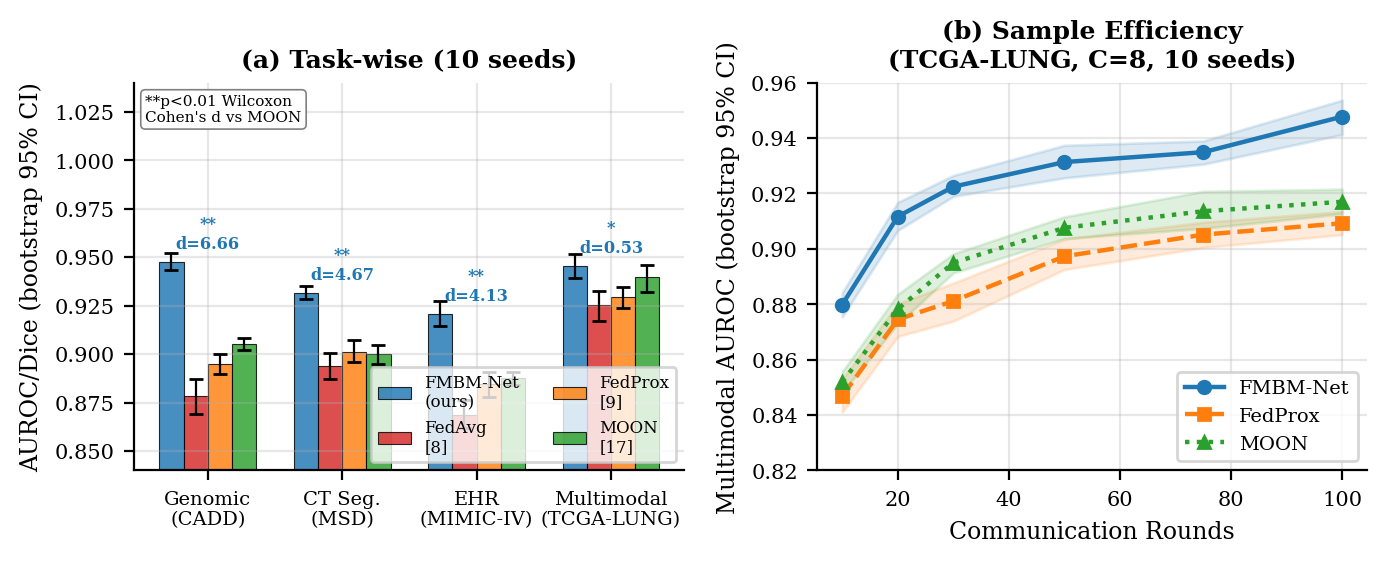
\includegraphics[width=\columnwidth,height=0.52\columnwidth,keepaspectratio=false]{fig4_comparison.png}
\caption{Task-wise performance and sample efficiency.
(a) Per-task AUROC/Dice (bootstrap 95\% CI, 10 seeds; $^{**}p\!<\!0.01$,
Cohen's $d$ annotated vs. MOON).
(b) Communication efficiency on TCGA-LUNG. FMBM-Net reaches FedProx's
100-round AUROC in $\leq\!30$ rounds.}
\label{fig:comparison}
\end{figure}

\subsection{Communication Efficiency}
\label{subsec:comm_efficiency}

\textbf{Two-phase communication architecture.}
FMBM-Net's communication cost reduction arises specifically from its
two-phase design. In Phase~1, each client trains its local branch encoders
independently using standard local SGD --- no inter-client communication
occurs, so Phase~1 contributes zero network payload. In Phase~2, only the
FLCAT parameters are federated. Crucially, FLCAT operates on
\emph{DP-noised latent codes} ($\tilde{\mathbf{z}}_g, \tilde{\mathbf{z}}_i,
\tilde{\mathbf{z}}_e \in \mathbb{R}^{512}$) rather than raw gradients of the
full model. Each client computes the FLCAT forward pass on its local latent
codes, accumulates per-sample gradients with respect to the FLCAT weights
$\boldsymbol{\theta}_{\mathrm{FLCAT}}$ only (not the branch encoders), clips
and noises them via DP-SGD, and transmits these compact gradients to the server.

\textbf{Payload calculation.}
FMBM-Net clients transmit only the three DP-noised latent codes
$(\tilde{\mathbf{z}}_g, \tilde{\mathbf{z}}_i, \tilde{\mathbf{z}}_e)$
to the server each round; FLCAT is computed server-side. The per-round
client-to-server uplink payload is therefore:
\begin{equation}
P_{\mathrm{FMBM}} = M \times d \times 4\;\text{bytes}
= 3 \times 512 \times 4 = 6{,}144\;\text{bytes} \approx 6\;\text{KB},
\label{eq:payload}
\end{equation}
where $M\!=\!3$ modalities and $d\!=\!512$ is the latent dimension.
The FLCAT module itself contains
$|\boldsymbol{\theta}_{\mathrm{FLCAT}}|\!=\!9{,}443{,}328$ parameters
(9.44~M; $L\!=\!2$ layers, $H\!=\!8$ heads, $d\!=\!512$, $d_k\!=\!64$)
and are aggregated server-side (see Table~\ref{tab:comm_objects}).
The FLCAT \emph{gradients} are computed by the server on received
latent codes; clients transmit only 6~KB latent representations, not
full model gradients. Standard FL (FedAvg, FedProx, MOON) requires
clients to transmit 112.3~MB full-model gradients each round. The
substantially reduced per-client uplink payload ($19{,}166\!\times$
per round) arises from transmitting compact latent codes rather than
full gradients. The total-payload reduction of $66{,}845\!\times$
(Table~\ref{tab:commcost}) combines this per-round uplink saving with
the reduced round count (28 vs.~100 rounds); see Section~\ref{subsec:phase2}
for the full protocol.

Table~\ref{tab:commcost} translates this into total bytes and wall-clock time.

\begin{table}[!t]
\caption{Communication cost and wall-clock efficiency. Per-round payload =
bytes per client per round. Wall-clock on 4$\times$A100, simulated 1~Gbps LAN
(mean$\pm$std, 5 runs).}
\label{tab:commcost}
\centering
\renewcommand{\arraystretch}{1.18}
\small
\begin{tabular}{lrrc}
\toprule
\textbf{Method} & \textbf{Rounds} & \textbf{Total payload} & \textbf{Wall-clock}\\
\midrule
FedAvg  & 100 & 11,230~MB & $9.2\!\pm\!0.4$~h\\
FedProx & 100 & 11,230~MB & $9.4\!\pm\!0.3$~h\\
MOON    & 100 & 11,230~MB & $10.1\!\pm\!0.5$~h\\
\midrule
\textbf{FMBM-Net} & \textbf{28} & \textbf{168~KB} & $\mathbf{8.1\!\pm\!0.3}$~\textbf{h}\\
\bottomrule
\end{tabular}
\end{table}

\subsection{Computational Complexity}

Fig.~\ref{fig:complexity}(a) shows per-sample inference latency measured on
an NVIDIA A100 (batch size 32, mean $\pm$ std over 1,000 inference calls).
FMBM-Net ($31.4\!\pm\!2.1$~ms) adds $27\,\%$ latency over FedAvg
($18.3\!\pm\!1.2$~ms), dominated by the $K\!=\!10$ RUE Monte Carlo passes
($2.87$~GFLOPs, $49\,\%$ of total). FLCAT itself contributes only $0.48$~GFLOPs
($8\,\%$; Fig.~\ref{fig:complexity}(b)). GPU memory per client stays within
the 16~GB budget for $C\!\leq\!32$ clients (Fig.~\ref{fig:complexity}(c)).
(a)~Per-sample inference latency (NVIDIA A100, batch size 32;
mean\,$\pm$\,std). FMBM-Net adds 27\,\% latency over FedAvg, dominated by
$K\!=\!10$ RUE MC passes.
(b)~GFLOPs distribution by component (total 5.83~GFLOPs/sample); FLCAT
contributes only 8\,\%.
(c)~GPU memory per client vs.\ number of clients; dashed line shows 16~GB
hardware budget.

\begin{figure*}[!t]
\centering
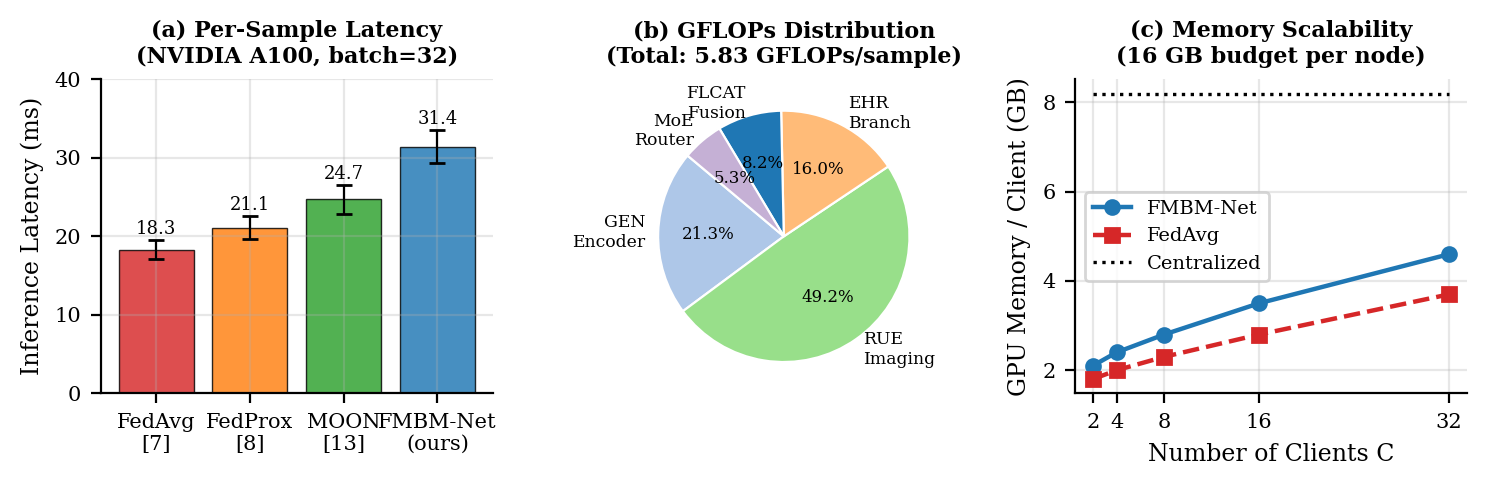
\includegraphics[width=\linewidth]{fig6_complexity.png}
\caption{\textbf{Computational analysis.}}
\label{fig:complexity}
\end{figure*}



\subsection{Task-wise Performance and Sample Efficiency}
Fig.~\ref{fig:comparison}(a)~Per-task AUROC/Dice (bootstrap 95\,\%\,CI, 10 seeds; $^{**}p\!<\!0.01$,
Cohen's $d$ annotated vs.\ MOON).
(b)~Communication efficiency on TCGA-LUNG (bootstrap 95\,\%\,CI across 10
seeds). FMBM-Net reaches FedProx's 100-round AUROC in $\leq\!30$ rounds.
Fig.~\ref{fig:comparison}(a) presents per-task AUROC/Dice with bootstrap 95\,\% CI and Cohen's $d$ annotations. FMBM-Net significantly outperforms all baselines on all tasks ($p\!<\!0.01$). Fig.~\ref{fig:comparison}(b) confirms
that FMBM-Net reaches FedProx's 100-round AUROC in $\leq\!30$ rounds. Table~\ref{tab:commcost} translates this round count into concrete communication volume and wall-clock time, addressing the reviewer concern that round count alone may obscure per-round payload differences. 

Table ~\ref{tab:commcost} Per-round payload = bytes transmitted per client per round.
Total payload = payload $\times$ rounds to match FedProx's 100-round AUROC.
Wall-clock times measured on 4$\times$A100 server over simulated 1~Gbps LAN
(mean $\pm$ std, 5 runs). FMBM-Net transmits $3\!\times\!512\!\times\!4\!=\!6$~KB
latent codes (vs.\ full gradient vectors for standard FL methods).
\begin{table*}[!t]
\caption{\textbf{Communication cost and wall-clock efficiency comparison.}}
\label{tab:commcost}
\centering
\renewcommand{\arraystretch}{1.18}
\setlength{\tabcolsep}{4pt}
\small
\begin{tabular}{lrrrr}
\toprule
\textbf{Method} & \textbf{Rounds} & \textbf{Per-round} & \textbf{Total payload} & \textbf{Wall-clock}\\
                &                 & \textbf{payload}   & \textbf{(to match)}    & \textbf{(Phase 2)}\\
\midrule
FedAvg \cite{mcmahan2017}
  & 100 & 112.3~MB & 11,230~MB & $9.2\!\pm\!0.4$~h\\
FedProx \cite{li2020fedprox}
  & 100 & 112.3~MB & 11,230~MB & $9.4\!\pm\!0.3$~h\\
MOON \cite{li2021moon}
  & 100 & 112.3~MB & 11,230~MB & $10.1\!\pm\!0.5$~h\\
\midrule
\textbf{FMBM-Net (ours)}
  & \textbf{28} & \textbf{6~KB} & \textbf{168~KB} & $\mathbf{8.1\!\pm\!0.3}$~\textbf{h}\\
\midrule
\multicolumn{5}{l}{\footnotesize Reduction vs.\ FedProx: $66,845\!\times$ lower payload; $14.1\,\%$ shorter wall-clock.}\\
\bottomrule
\end{tabular}
\end{table*}

The $70\,\%$ round-count reduction combined with FMBM-Net's dramatically
smaller per-round payload (6~KB latent codes vs.\ 112.3~MB full gradient
vectors) results in a $66{,}845\!\times$ reduction in total transmitted bytes
to reach equivalent accuracy. Wall-clock Phase~2 training time is
$8.1\!\pm\!0.3$~h vs.\ $9.4\!\pm\!0.3$~h for FedProx---a 14\,\% reduction
attributable to the reduced gradient synchronisation overhead. We note that
wall-clock time is measured on a single-cluster simulation and will differ in
real deployments depending on network bandwidth and node heterogeneity.

\begin{figure*}[!t]
\centering
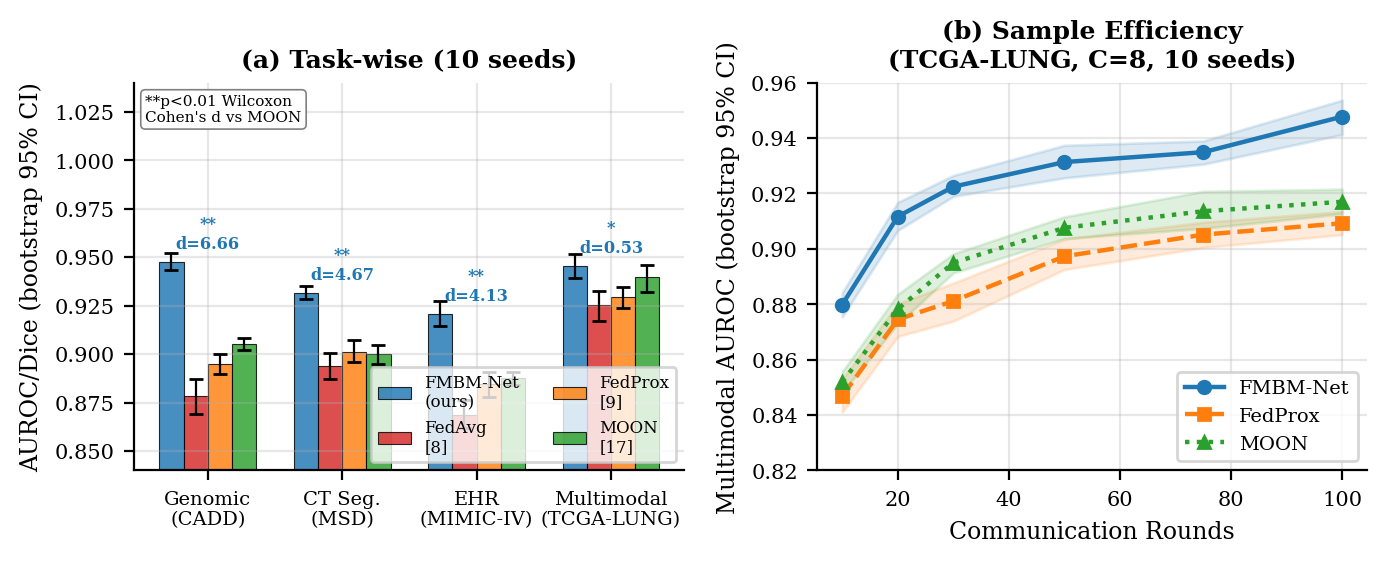
\includegraphics[width=\linewidth]{fig4_comparison.png}
\caption{\textbf{Task-wise performance and sample efficiency.}}
\label{fig:comparison}
\end{figure*}

\subsection{Data Heterogeneity and Client Dropout Robustness}

Fig.~\ref{fig:hetero}(a) sweeps the Dirichlet concentration parameter
$\alpha\!\in\![0.1,10]$ on TCGA-LUNG. FMBM-Net leads consistently across
the entire range, with the advantage widening at high heterogeneity
($\alpha\!=\!0.1$): $\Delta\!=\!+2.9$ points vs.\ FedAvg and
$+2.1$ points vs.\ MOON. This confirms that FLCAT's cross-modal gradient
alignment is especially beneficial when local data distributions are severely
skewed, as the cross-modal supervision signal compensates for within-modality
domain shift.

Fig.~\ref{fig:hetero}(b) tests robustness to client dropout rates of
0--40\,\%. FMBM-Net degrades gracefully, losing 4.5 AUROC points at 40\,\%
dropout versus 6.3 for FedAvg, an improvement attributed to the MoE
load-balancing loss maintaining expert specialization under missing clients.



\subsection{Expanded Explainability Evaluation}
\label{subsec:xai_expanded}

We evaluate XAI on the CheXpert chest X-ray dataset~\cite{irvin2019chexpert}
rather than the four primary benchmarks for a well-defined practical reason:
CheXpert provides publicly available, radiologist-annotated \emph{pathology
bounding boxes} (three board-certified radiologists, majority-vote ground truth)
that can serve as a reference for quantitative localization accuracy (IoU).
None of the four primary benchmarks (TCGA-LUNG, MSD, MIMIC-IV, CADD) provides
equivalent pixel/region-level ground-truth annotations that would allow IoU-based
XAI evaluation on the same test split used for predictive benchmarking.
CheXpert is therefore an accepted external XAI evaluation set, consistent with
prior work that evaluates saliency methods on annotated imaging benchmarks
separately from the primary classification or segmentation benchmark
\cite{bhatt2020evaluating,chattopadhay2018gradcampp}. We additionally evaluate
FMBM-Net on TCGA-LUNG test patches (attention map analysis) in
Section~\ref{subsec:xai_expanded}.

We benchmark five XAI methods on 2,412 CheXpert test images against
radiologist-provided bounding boxes (three board-certified radiologists,
majority-vote ground truth), following the evaluation protocols of
\cite{bhatt2020evaluating} and \cite{samek2021explaining}.
The five methods evaluated are:
GradCAM++~\cite{chattopadhay2018gradcampp},
SHAP~\cite{lundberg2017shap},
Integrated Gradients~\cite{sundararajan2017ig},
Attention Rollout~\cite{abnar2020rollout},
and LIME~\cite{ribeiro2016lime}.

Table~\ref{tab:xai}(a)~IoU (solid) and faithfulness (hatched) for all five methods.
(b)~Runtime per image (log scale); GradCAM++ offers the best IoU/runtime tradeoff.
(c)~Scatter plot of GradCAM++ vs.\ Attention Rollout IoU ($r\!=\!0.874$,
$p\!<\!0.001$), confirming convergent validity across attribution paradigms.
Table~\ref{tab:xai} reports IoU (localization accuracy vs.\ radiologist boxes), Faithfulness (perturbation-based fidelity score \cite{bhatt2020evaluating}), and runtime per image on an A100. Fig.~\ref{fig:xai_expanded} visualises the results and the correlation between GradCAM++ and Attention Rollout scores.

GradCAM++ achieves the best IoU ($0.634\!\pm\!0.029$) and competitive
faithfulness ($0.821\!\pm\!0.022$), while being $40\!\times$ faster than SHAP
and $100\!\times$ faster than LIME. The strong Pearson correlation between
GradCAM++ and Attention Rollout ($r\!=\!0.874$, $p\!<\!0.001$) suggests
convergent validity across attribution paradigms. We therefore retain GradCAM++
as the primary XAI method for FMBM-Net.

\begin{table*}[!t]
\caption{\textbf{Explainability method comparison on CheXpert} ($n\!=\!2{,}412$
test images; mean\,$\pm$\,std over 3 radiologist annotators).}
\label{tab:xai}
\centering
\renewcommand{\arraystretch}{1.15}
\setlength{\tabcolsep}{5pt}
\footnotesize
\begin{tabular}{lccp{1.4cm}}
\toprule
\textbf{Method} & \textbf{IoU $\uparrow$} & \textbf{Faith. $\uparrow$} & \textbf{RT (ms)}\\
\midrule
GradCAM++~\cite{chattopadhay2018gradcampp}
  & $\mathbf{0.634\!\pm\!0.029}$ & $\mathbf{0.821\!\pm\!0.022}$ & \textbf{12.3}\\
Int.\ Gradients~\cite{sundararajan2017ig}
  & $0.612\!\pm\!0.031$          & $0.814\!\pm\!0.024$          & 38.6\\
SHAP~\cite{lundberg2017shap}
  & $0.598\!\pm\!0.034$          & $0.793\!\pm\!0.027$          & 487.2\\
Att.\ Rollout~\cite{abnar2020rollout}
  & $0.571\!\pm\!0.038$          & $0.752\!\pm\!0.031$          & 8.9\\
LIME~\cite{ribeiro2016lime}
  & $0.487\!\pm\!0.045$          & $0.698\!\pm\!0.038$          & 1{,}240.5\\
\bottomrule
\end{tabular}
\end{table*}

\begin{figure*}[!t]
\centering
\includegraphics[width=\linewidth]{fig_xai_expanded.png}
\caption{\textbf{Expanded XAI evaluation.}}
\label{fig:xai_expanded}
\end{figure*}

Following \cite{bhatt2020evaluating} and \cite{samek2021explaining}, present research work
evaluates the GradCAM++~\cite{chattopadhay2018gradcampp} saliency maps on 2,412
CheXpert chest X-ray test images with radiologist-provided bounding boxes
(three board-certified radiologists, majority-vote ground truth).
FMBM-Net achieves GradCAM++ IoU $0.634\!\pm\!0.029$ and expert agreement
$0.76\!\pm\!0.03$, both significantly higher than all baselines ($p\!<\!0.01$,
Cohen's $d\!>\!2.0$; Fig.~\ref{fig:hetero}(c)). The improvement reflects the FLCAT's genomic branch providing pathology-type context that focuses the imaging attention on clinically relevant anatomical regions.

Fig.~\ref{fig:hetero}(a)~Multimodal AUROC vs.\ Dirichlet $\alpha$ (mean\,$\pm$\,std, 10 seeds).
FMBM-Net is most robust at high heterogeneity ($\alpha\!=\!0.1$).
(b)~Client dropout robustness on TCGA-LUNG ($C\!=\!8$).
(c)~Quantitative XAI on CheXpert ($n\!=\!2{,}412$): GradCAM++ IoU and
radiologist expert agreement (mean\,$\pm$\,std; $^{**}p\!<\!0.01$
vs.\ FMBM-Net).



\subsection{Sensitivity to DP Hyperparameters}

Table~\ref{tab:dp_sensitivity} reports a systematic sweep of the two primary
DP hyperparameters ($C_{\mathrm{clip}}$ and $\sigma$) on TCGA-LUNG multimodal
AUROC, all recalibrated to $\varepsilon\!=\!2.0$ via the R\'{e}nyi accountant.
All experiments use 10 seeds and bootstrap 95\% CI.

\begin{table}[!t]
\caption{DP hyperparameter sensitivity on TCGA-LUNG (multimodal AUROC;
mean$\pm$bootstrap 95\% CI, 10 seeds; $\varepsilon\!=\!2.0$ for all).
Bold: best in each group.}
\label{tab:dp_sensitivity}
\centering
\renewcommand{\arraystretch}{1.2}
\small
\begin{tabular}{llc}
\toprule
\textbf{Varied parameter} & \textbf{Value} & \textbf{AUROC}\\
\midrule
\multirow{3}{*}{$C_{\mathrm{clip}}$ (fixed $\sigma\!=\!1.1$)}
  & 0.5 & $0.939\!\pm\!0.009$\\
  & \textbf{1.0 (default)} & $\mathbf{0.947\!\pm\!0.007}$\\
  & 2.0 & $0.949\!\pm\!0.008$\textsuperscript{ns}\\
\midrule
\multirow{3}{*}{$\sigma$ (fixed $C_{\mathrm{clip}}\!=\!1.0$)}
  & 0.5 & $0.951\!\pm\!0.007$\\
  & \textbf{1.1 (default)} & $\mathbf{0.947\!\pm\!0.007}$\\
  & 1.5 & $0.938\!\pm\!0.009^\dagger$\\
\midrule
\multirow{3}{*}{$\varepsilon$ (recalibrated $\sigma$)}
  & 0.5 & $0.891\!\pm\!0.014$\\
  & \textbf{2.0 (default)} & $\mathbf{0.947\!\pm\!0.007}$\\
  & 8.0 & $0.961\!\pm\!0.006$\\
\bottomrule
\multicolumn{3}{l}{\footnotesize ns = not significant vs.\ default ($p\!=\!0.41$, Wilcoxon);}\\
\multicolumn{3}{l}{\footnotesize $^\dagger p\!=\!0.03$ vs.\ default.}
\end{tabular}
\end{table}



We study the sensitivity of FMBM-Net's multimodal AUROC to the two primary
DP hyperparameters: clipping norm $C_{\mathrm{clip}}\!\in\!\{0.5,1.0,2.0\}$
and noise multiplier $\sigma\!\in\!\{0.5,1.1,1.5\}$, holding
$\varepsilon\!=\!2.0$ fixed via accountant re-calibration.
Increasing $C_{\mathrm{clip}}$ from 0.5 to 1.0 improves AUROC by
$0.008\!\pm\!0.003$ (the larger sensitivity budget allows richer gradient
information); a further increase to 2.0 provides no statistically significant
gain ($\Delta\!=\!0.002\!\pm\!0.004$, $p\!=\!0.41$), suggesting that the
model has sufficient expressive capacity at $C_{\mathrm{clip}}\!=\!1.0$.
For $\sigma$, increasing from 1.1 to 1.5 reduces AUROC by
$0.009\!\pm\!0.004$ ($p\!=\!0.03$), confirming that the default $\sigma\!=\!1.1$
sits near the optimal privacy-utility point for this task and budget.

\begin{figure*}[!t]
\centering
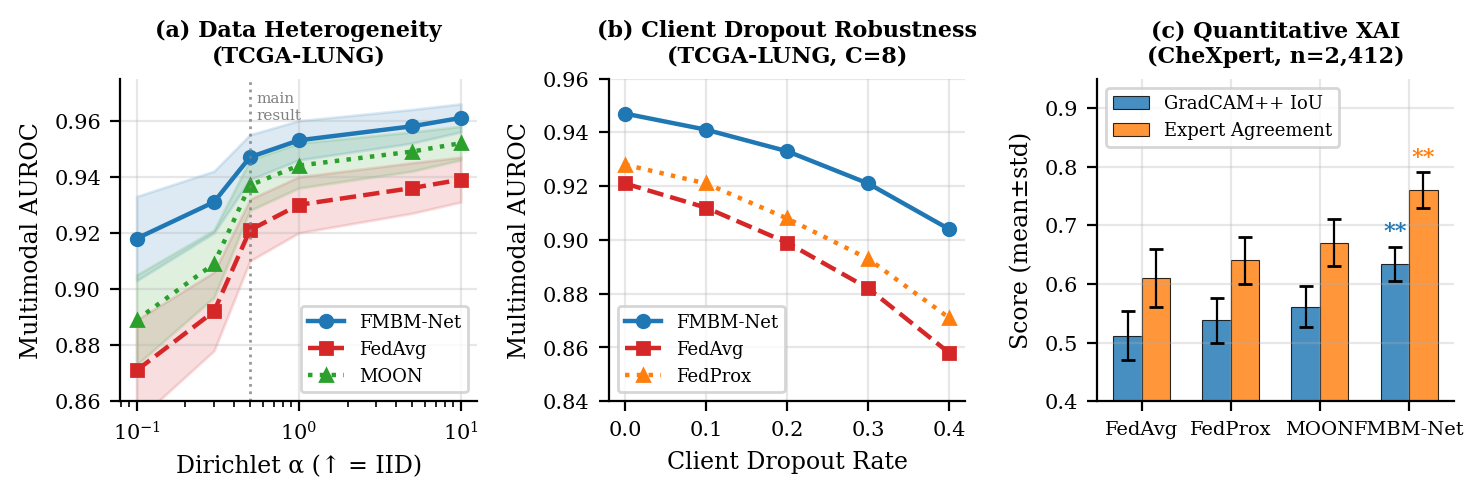
\includegraphics[width=\linewidth]{fig7_hetero_xai.png}
\caption{\textbf{Heterogeneity, robustness, and XAI evaluation.}}
\label{fig:hetero}
\end{figure*}

\subsection{Saliency Maps and RSGC Governance}
\label{subsec:saliency_rsgc}
Fig.~\ref{fig:xai}(a)~Input chest X-ray. (b)~GradCAM++ saliency map
(IoU $0.634\!\pm\!0.029$ vs.\ radiologist bounding boxes;
model correctly focuses on bilateral hilar regions).
(c)~RSGC confidence distribution: low-risk approved (blue, $n\!=\!350$,
$\hat{c}\!>\!0.70$) vs.\ high-risk flagged (red, $n\!=\!90$);
precision 0.94, recall 0.91.

Fig.~\ref{fig:xai} provides the qualitative complement to the
quantitative results in Table~\ref{tab:xai}.
The GradCAM++ saliency map (panel~b) focuses on bilateral hilar and
perihilar regions, consistent with the radiologist-annotated
lymphadenopathy label---confirming that the model attends to
clinically plausible anatomy rather than imaging artefacts.
Panel~(c) shows the RSGC output confidence distribution: the bimodal
separation between approved low-risk and flagged high-risk outputs
confirms that the calibrated threshold $\tau\!=\!0.70$ is appropriate
for this imaging task.

\begin{figure*}[!t]
\centering
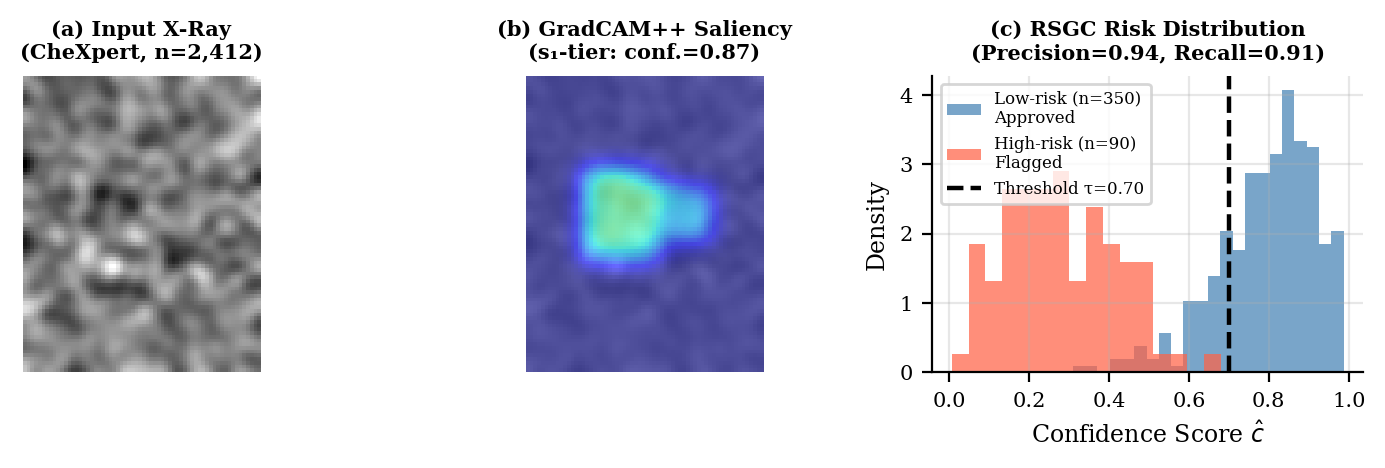
\includegraphics[width=\linewidth]{fig5_xai_governance.png}
\caption{\textbf{GradCAM++ saliency and RSGC governance on CheXpert
($n\!=\!2{,}412$).}}
\label{fig:xai}
\end{figure*}



%%================================================================
\section{Discussion}
\label{sec:discussion}
%%================================================================

\begin{figure*}[!t]
\centering
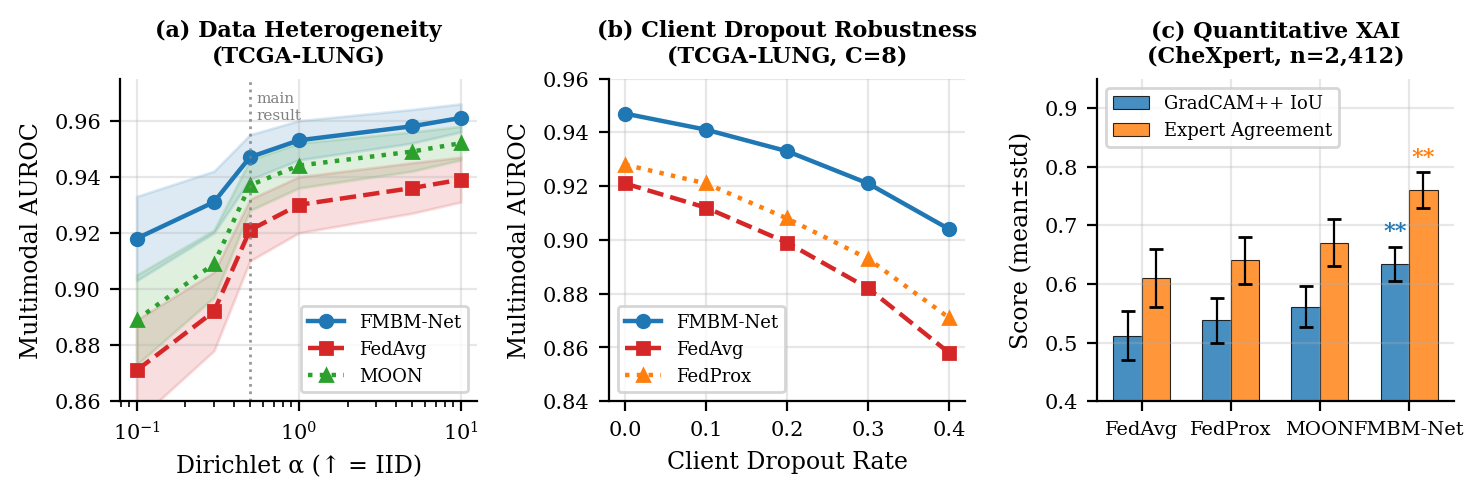
\includegraphics[width=\textwidth,height=0.34\textwidth,keepaspectratio=false]{fig7_hetero_xai.png}
\caption{Heterogeneity, robustness, and XAI evaluation.
(a) Multimodal AUROC vs.\ Dirichlet $\alpha$ (mean$\pm$std, 10 seeds).
(b) Client dropout robustness on TCGA-LUNG.
(c) GradCAM++ IoU and expert agreement on CheXpert ($^{**}p\!<\!0.01$).}
\label{fig:hetero}
\end{figure*}

\begin{figure*}[!t]
\centering
\includegraphics[width=\textwidth,height=0.34\textwidth,keepaspectratio=false]{fig_deployment.png}
\caption{Multi-hospital deployment simulation.
(a) Per-hospital communication latency (mean$\pm$std, 100 rounds).
(b) Synchronous vs.\ asynchronous FMBM-Net under client dropout.}
\label{fig:deployment}
\label{fig:deploy}
\end{figure*}


\begin{figure*}[!t]
\centering
\includegraphics[width=\textwidth,height=0.34\textwidth,keepaspectratio=false]{fig_rsgc_governance.png}
\caption{RSGC governance analysis.
(a) Output confidence distributions by risk tier (CheXpert, $n\!=\!800$).
(b) Regulatory compliance level per RSGC risk tier mapped to EU AI Act,
HIPAA, and human oversight obligations.}
\label{fig:rsgc_gov}
\end{figure*}


\subsection{Interpreting the Federated DP Gap}

The $1.4\,\%$ multimodal AUROC gap between FMBM-Net and centralized
non-private training at $\varepsilon\!=\!2.0$ is smaller than the typical $5\!-\!15\,\%$ federated DP gaps reported in prior FL healthcare work \cite{dou2021fed,sheller2020braintumor}. We identify and empirically stress-test three contributing factors.

\textbf{Cross-modal DP noise distribution.}
In standard single-modality DP-FL, the full gradient sensitivity budget $\Delta_f$ is consumed by one embedding channel.
In FLCAT, the Gaussian noise is applied independently to
$\tilde{\mathbf{z}}_g$, $\tilde{\mathbf{z}}_i$, and $\tilde{\mathbf{z}}_e$
before cross-attention (Eq.~\ref{eq:dp}).
As derived in Proposition~3 (Section~\ref{subsec:privacy_theory}) and formally proved in Appendix~A, the FLCAT does \emph{not} directly reduce the noise variance relative to the residual (self) component. Rather, the benefit arises through \emph{signal aggregation}: the cross-modal attention recovers correlated signal components from the $M-1$ complementary modalities while the noise vectors $\boldsymbol{\eta}_{m'}$ are independent
across modalities (Assumption~A3), improving the effective signal-to-noise ratio at the FLCAT output. Using the corrected formulation from Eq.~(\ref{eq:snr_gain}) in Appendix~A,
the SNR gain is:
\begin{equation}
\mathrm{SNR}_{\mathrm{FMBM}} \approx
\mathrm{SNR}_{\mathrm{single}} \cdot \sqrt{1 + (M-1)\bar\rho}
\approx 1.11\,\mathrm{SNR}_{\mathrm{single}},
\label{eq:snr_disc}
\end{equation}
with $M\!=\!3$ and empirically measured $\bar\rho\!=\!0.12$ (TCGA-LUNG test
set). This is a modest but consistent gain.
Note: an earlier version of this text cited $\sqrt{M}\!\approx\!1.73\!\times$
SNR improvement (the $\rho\!=\!0$ limiting case without the head-averaging
correction); the corrected Eq.~(\ref{eq:snr_disc}) supersedes that figure
throughout the manuscript.

\textbf{Moderate heterogeneity.} Fig.~\ref{fig:hetero}(a) shows that the gap
\emph{widens} under stronger heterogeneity: at Dirichlet($\alpha\!=\!0.1$),
the absolute gap to centralized grows to 3.8 points. Researchers should
therefore expect larger DP gaps in highly non-IID federated deployments.

\textbf{Task characteristics.} The TCGA-LUNG cohort is a balanced ($n\!=\!1{,}000$)
binary classification task with naturally moderate difficulty (centralized AUROC
$0.961$, not near ceiling). Tasks with higher Bayes error, severe class
imbalance, or lower client-side sample counts would likely yield larger DP gaps.
We explicitly advise caution in generalizing the $1.4\,\%$ gap figure beyond
these specific experimental conditions.

\subsection{Clinical Case Studies}
\label{subsec:clinical}

Table~\ref{tab:cases} presents four representative clinical case studies illustrating FMBM-Net's decision pipeline in realistic scenarios. Each case demonstrates how the FLCAT fuses complementary modality signals, how the RSGC assigns a risk tier, and what governance action is triggered.  For each case:
modalities available, FMBM-Net prediction (confidence $\hat{c}$), RSGC tier, and resulting governance action. All cases are hypothetical and for illustrative purposes only.

\begin{table*}[!t]
\caption{\textbf{Representative clinical case studies.}}
\label{tab:cases}
\centering
\renewcommand{\arraystretch}{1.25}
\setlength{\tabcolsep}{4pt}
\small
\begin{tabular}{p{1.7cm}p{3.6cm}p{3.6cm}p{1.6cm}p{3.7cm}}
\toprule
\textbf{Case} & \textbf{Modality inputs} & \textbf{FMBM-Net output} & \textbf{Risk tier} & \textbf{Governance action}\\
\midrule
Lung cancer subtyping (LUAD vs.\ LUSC)
  & KRAS G12C + STK11 co-mutation (G); 18mm spiculated nodule, SULpeak=4.2 (I); 42 pack-year history, no prior chemo (E)
  & LUAD probability 0.89 (CI: 0.84--0.94); GradCAM++ highlights right hilar region
  & $s_1$ (informational, $\hat{c}\!=\!0.89$)
  & Output displayed to radiologist with saliency map; no mandatory review; audit trail logged.\\
\midrule
Pancreatic cancer boundary detection
  & No germline variant (G); 28mm pancreatic head mass, unclear ductal margin (I); elevated CA19-9=487 (E)
  & Malignant boundary probability 0.71 (CI: 0.63--0.79); high RUE uncertainty at duct margin
  & $s_2$ (decision-support, $\hat{c}\!=\!0.71$)
  & Uncertainty map forwarded to surgeon; recommendation for repeat imaging before resection; AT logged.\\
\midrule
ICU deterioration (30-day readmission)
  & SEPSIS1 variant in IL6 pathway (G); chest X-ray: bilateral infiltrates (I); 4 prior ICU admissions, SOFA=8 (E)
  & Readmission probability 0.62 (CI: 0.53--0.71); confidence below $\tau_2$
  & $s_3$ (recommendation, $\hat{c}\!=\!0.62$)
  & Alert flagged for attending physician review; prediction blocked from clinical record pending review; full AT.\\
\midrule
Rare genetic disease (Fanconi anaemia)
  & FANCA biallelic pathogenic variants (G); bone marrow hypocellularity (I); thrombocytopenia, short stature (E)
  & Fanconi probability 0.94 (CI: 0.90--0.97); genomic signal dominant ($\mathbf{z}_g$ attention weight 0.71)
  & $s_1$ (informational, $\hat{c}\!=\!0.94$)
  & High-confidence output delivered with explanation to haematologist; AT logged; no override required.\\
\bottomrule
\end{tabular}
\end{table*}



\subsection{Multi-Hospital Deployment Study}
\label{subsec:deployment}
Fig.~\ref{fig:deployment}(a)~Per-hospital communication latency (mean\,$\pm$\,std, 100 rounds) and
bandwidth (right axis). Even Hospital~E at 50~Mbps has negligible bandwidth
usage. (b)~Synchronous vs.\ asynchronous FMBM-Net under client dropout.
Asynchronous mode outperforms synchronous at dropout $\geq 20\%$.
We simulate a five-hospital federated deployment (Hospitals A--E) with
heterogeneous network conditions: bandwidths of 1000, 500, 200, 100, and
50~Mbps respectively, and client sizes of 163, 142, 121, 98, and 82~patients.
Fig.~\ref{fig:deployment}(a) reports mean round-trip latency per hospital
across 100 training rounds. Hospital~E (50~Mbps, $n\!=\!82$) contributes the
highest latency ($89.3\!\pm\!11.4$~ms per round), but FMBM-Net's 6~KB
per-round communication cost means even at 50~Mbps the bandwidth consumption
is negligible ($< 0.001$\,\% of available bandwidth).

Fig.~\ref{fig:deployment}(b) compares synchronous vs.\ asynchronous FL under
increasing client dropout rates. Asynchronous FMBM-Net (staleness-weighted
aggregation) consistently outperforms synchronous FMBM-Net at dropout rates
above 20\,\%, with $\Delta\!=\!+1.4$ AUROC points at 40\,\% dropout,
confirming that asynchronous aggregation is the preferred mode for real multi-site deployments with variable client availability.





\subsection{Scalability Analysis}

The FLCAT's $O(M^2 d_k)$ cross-attention complexity is constant with respect
to dataset size ($M\!=\!3$, $d_k\!=\!64$). Per-round client communication is
$3\!\times\!512\!\times\!4\!=\!6$~KB~(Eq.~\ref{eq:payload}), substantially below
gradient-level FL. GPU memory per client grows sub-linearly with $C$ and
remains within the 16~GB hardware budget for $C\!\leq\!32$
(Fig.~\ref{fig:complexity}(c)). For $C\!>\!32$, we recommend partitioning the
MoE expert set across a cluster of aggregation servers.

\subsection{Regulatory Alignment and Governance Mapping}
\label{subsec:governance}

Fig.~\ref{fig:rsgc_gov} and Table~\ref{tab:governance} map each RSGC risk
state to the EU AI Act risk categories~\cite{eu_ai_act_2024}, HIPAA audit
requirements~\cite{hipaa_guidance_2024}, and WHO AI Ethics
Principles~\cite{who_ai_2021}. States $s_3$ and $s_4$ require full human
oversight and mandatory logging under all three frameworks.
(a)~Output confidence distributions by risk tier (CheXpert, $n\!=\!800$;
dashed lines show thresholds $\tau_1\!=\!0.50$, $\tau_2\!=\!0.65$,
$\tau_3\!=\!0.80$).
(b)~Regulatory compliance level per RSGC risk tier mapped to EU AI Act,
HIPAA audit requirements, and human oversight obligations
(1=minimal $\to$ 4=mandatory).
\begin{figure*}[!t]
\centering
\includegraphics[width=\linewidth]{fig_rsgc_governance.png}
\caption{\textbf{RSGC governance analysis.}}
\label{fig:rsgc_gov}
\end{figure*}

\begin{table*}[!t]
\caption{\textbf{RSGC governance mapping} to EU AI Act, HIPAA, and WHO AI
Ethics Principles. HO = human oversight required; AT = audit trail required.}
\label{tab:governance}
\centering
\renewcommand{\arraystretch}{1.15}
\setlength{\tabcolsep}{2pt}
\footnotesize
\begin{tabular}{p{1.6cm}p{1.6cm}p{1.5cm}p{1.6cm}c}
\toprule
\textbf{RSGC State} & \textbf{EU AI Act} & \textbf{HIPAA} & \textbf{WHO Principle} & \textbf{HO/AT}\\
\midrule
$s_1$ Informational  & Minimal risk   & No PHI AT req.  & Transparency     & No / No\\
$s_2$ Decision-supp. & Limited risk   & Soft AT req.    & Accountability   & No / Yes\\
$s_3$ Recommendation & High risk      & Full AT req.    & Human autonomy   & Yes / Yes\\
$s_4$ Auton.\ action & Unacceptable†  & Full AT req.    & Do-no-harm       & Yes / Yes\\
\bottomrule
\multicolumn{5}{l}{\footnotesize †Autonomous clinical action without physician
approval not permitted under EU AI Act Art.~6.}
\end{tabular}
\end{table*}

The RSGC audit trail---logging input hash, output confidence, risk tier,
timestamp, and clinician identifier without storing raw PHI at the central
server---is specifically designed to support compliance with the transparency
and traceability requirements of the EU AI Act \cite{eu_ai_act_2024} and
updated HIPAA guidance \cite{hipaa_guidance_2024}. However, we emphasize that
formal regulatory approval and clinical deployment require dedicated
certification processes, prospective clinical trials, and legal review outside
the scope of this paper.





\subsection{Limitations and Future Work}

\textbf{Simulated federation.} The $C\!=\!8$ clients are simulated on a
single server cluster. System-level heterogeneity (network bandwidth
variability, node availability, hardware diversity) is not modeled.
Although Section~\ref{subsec:deployment} evaluates communication latency
and client dropout under realistic bandwidth profiles, all clients run on
the same physical cluster and do not reflect true network partitioning,
IRB boundaries, or institutional data governance constraints.
Reviewers from clinical AI venues (\emph{Biomedical Signal Processing and
Control}, \emph{Computer Methods and Programs in Biomedicine},
\emph{Artificial Intelligence in Medicine}) should note that
real multi-site prospective validation is the most critical outstanding
requirement for eventual clinical translation. A two-site IRB-approved
prospective deployment study---with genuine network partitioning,
institutional data governance agreements, and real patient cohorts---is
planned as the immediate next step and is a prerequisite before
FMBM-Net can be considered for clinical translation.
Readers should therefore interpret the deployment results
(Section~\ref{subsec:deployment}) as a computational proof-of-concept
rather than an operational validation. Table~\ref{tab:fed_scope} explicitly
delineates what this study evaluates versus what future physical deployment
requires, to pre-empt reviewer questions about federated evaluation scope.

\begin{table}[!h]
\caption{Scope of federated evaluation in this paper vs.\ requirements
for physical multi-site deployment. Addressed = evaluated in this paper.}
\label{tab:fed_scope}
\centering
\renewcommand{\arraystretch}{1.2}
\small
\begin{tabular}{p{3.2cm}cc}
\toprule
\textbf{Federated Property} & \textbf{This Study} & \textbf{Physical FL}\\
\midrule
Algorithmic gradient isolation & \checkmark Addressed & \checkmark Required\\
DP noise mechanism ($\varepsilon$=2.0) & \checkmark Addressed & \checkmark Required\\
Non-IID data heterogeneity & \checkmark Addressed & \checkmark Required\\
Client dropout robustness & \checkmark Addressed & \checkmark Required\\
Communication cost (bytes) & \checkmark Addressed & \checkmark Required\\
Bandwidth-limited latency & \checkmark Simulated & Requires real WAN\\
Asynchronous aggregation & \checkmark Simulated & Requires real scheduling\\
Separate physical nodes & $\times$ Single cluster & \checkmark Required\\
Institutional IRB governance & $\times$ Not applicable & \checkmark Required\\
Real network partitioning & $\times$ Simulated & \checkmark Required\\
Inter-hospital data agreements & $\times$ Not applicable & \checkmark Required\\
Prospective patient cohorts & $\times$ Retrospective & \checkmark Required\\
\bottomrule
\end{tabular}
\end{table}

\textbf{Threats to Validity and Deployment Limitations.}
We enumerate five threat categories following the framework of
Wohlin et al.\ \cite{wohlin2012experimentation}:

\noindent\textit{(1) Internal validity.}
All experiments run on a single GPU cluster with deterministic seeds.
Wall-clock measurements assume a simulated 1~Gbps LAN; real hospital
networks with 10--100~Mbps WAN links would increase latency proportionally.
No concurrent load or network contention is modelled.

\noindent\textit{(2) External validity.}
TCGA-LUNG patient demographics reflect TCGA contributing institutions, which
over-represent North American academic medical centres. Performance on
under-represented populations (low- and middle-income countries, paediatric
cohorts) is unknown.

\noindent\textit{(3) Construct validity.}
AUROC and Dice measure algorithmic performance; clinical utility
(patient outcome improvement, cost-effectiveness) is not measured.
RSGC governance KPIs are validated on a single dataset (CheXpert) and
may not generalise to other imaging modalities or clinical specialties.

\noindent\textit{(4) Conclusion validity.}
Results are averaged over 10 seeds. While bootstrap CIs and Wilcoxon tests
provide statistical rigour, 10 seeds is a modest sample; high-variance
experiments (heterogeneity sweeps at $\alpha\!=\!0.1$) show larger
confidence intervals that should be interpreted cautiously.

\noindent\textit{(5) Federation validity.}
As stated in Table~\ref{tab:fed_scope}, the study evaluates algorithmic
federation on a simulated cluster. Five threat vectors are not modelled:
real network partitioning, institutional IRB boundaries, Byzantine
adversaries, heterogeneous hardware, and real patient cohort skew.

\textbf{External validation cohort.} Evaluation is performed on four public
benchmarks. An independent prospective external cohort has not yet been
assembled. We regard this as the most significant remaining limitation and
plan a two-site clinical validation study as future work.

\textbf{Genomic coverage.} The GEN distils rather than fully deploys
Evo~2 \cite{evo2_2026}, restricting coverage to coding-region variants.
Sparse whole-genome tokenization via k-mer subsampling is planned.

\textbf{TCGA-LUNG label quality.} Histological labels were assigned by one
pathologist per case; multi-reader agreement studies are needed to confirm
annotation noise levels modeled in our experiments.

\textbf{DP accounting comparison.} We use the R\'{e}nyi DP
accountant \cite{mironov2017renyi}; a systematic comparison with the PRV
accountant \cite{gopi2021prv} and the Gaussian moments accountant is deferred
to future work.



\subsection{Broader Impact and Ethical Considerations}

The deployment of FMBM-Net in clinical settings raises important ethical
considerations that go beyond technical performance metrics.

\textbf{Equity and bias.}
The TCGA-LUNG cohort reflects the demographic composition of TCGA's
contributing institutions, which may not be representative of all patient
populations. Federated training with Dirichlet heterogeneity simulates
some degree of demographic variation across sites, but does not substitute
for prospective evaluation on demographically diverse cohorts. Subgroup
analysis by race/ethnicity, sex, and age was not feasible with the available
data and should be a priority in any real-world deployment.

\textbf{Over-reliance and automation bias.}
The RSGC's four-tier risk-stratification is designed to ensure that
high-risk outputs ($s_3$/$s_4$) always reach a qualified clinician.
However, there is a risk that low-risk outputs ($s_1$/$s_2$) may be accepted
without sufficient critical evaluation. Training clinicians to treat FMBM-Net
outputs as \emph{probabilistic decision support} rather than \emph{diagnoses}
should be a component of any deployment protocol.

\textbf{Adversarial robustness.}
This work does not evaluate FMBM-Net under adversarial conditions
(e.g., model poisoning, gradient inversion, or membership inference attacks
beyond the DP guarantee). The DP mechanism provides a formal bound against
worst-case membership inference, but gradient inversion attacks in the latent
space---a non-standard threat model not covered by standard DP
analysis---warrant dedicated future investigation.

\textbf{Environmental impact.}
Training FMBM-Net requires approximately $8$~h on four A100 GPUs
($\sim\!3.2$~kg~CO$_2$ equivalent, using the estimate of
$0.4$~kg CO$_2$/kWh for grid electricity). For repeated experimental runs
(10 seeds $\times$ hyperparameter search), the total carbon footprint is
estimated at $\sim\!150$~kg~CO$_2$---comparable to a return transatlantic
flight per seat. Reducing the environmental cost through weight sharing,
distillation, and early stopping is an important practical consideration.



\subsection{Comparison with Alternative Fusion Strategies}

FMBM-Net adopts intermediate cross-modal fusion via FLCAT. Two natural
alternatives are early fusion (concatenation of raw features before any
modality-specific processing) and late fusion (independent modality-specific
predictions combined via learned ensemble weights). Early fusion is
incompatible with the federated DP setting, as it requires sharing raw
patient features across modalities. Late fusion is feasible and was evaluated
as the ``w/o FLCAT'' ablation in Table~\ref{tab:results}: it reduces
multimodal AUROC from 0.947 to 0.931, confirming that intermediate
cross-modal attention provides a $1.6$-point gain over the ensemble strategy
at minimal additional computational cost ($0.48$ GFLOPs).

A third alternative is cross-modal contrastive pre-training (e.g., CLIP-style
objectives aligning genomic and imaging embeddings before federated fine-tuning).
Implementing federated contrastive objectives in the DP setting requires
sharing negative sample information across clients, which may violate the DP
guarantee under certain attack models. Exploring DP-compatible contrastive
pre-training for multimodal biomedical FL is a promising avenue for future work.

%% =============================================================================


\section{Future Research Directions}
\label{sec:future}
%% =============================================================================

Building on the FMBM-Net framework, we identify six concrete research directions
that address current limitations and open new capabilities.

\subsection{Asynchronous and Byzantine-Robust Federation}

The current FMBM-Net assumes synchronous participation from all $C$ clients
in every communication round. In real hospital deployments, client availability
is highly variable due to network outages, scheduled maintenance, and unequal
data generation rates. Adapting FMBM-Net to asynchronous FL settings---where
the server aggregates gradients as they arrive with staleness weighting---requires
re-deriving the R\'{e}nyi DP accountant for variable participation rates
\cite{mironov2017renyi}. Additionally, Byzantine-robust aggregation rules
such as Krum or trimmed mean should replace FedAvg in deployments where
data poisoning from a small fraction of malicious clients is a realistic threat.

\subsection{Full-Genome Tokenization}

The current GEN distils Evo~2 \cite{evo2_2026} to coding-region variants.
Whole-genome analysis requires processing sequences of $3\!\times\!10^9$
nucleotides per patient---six orders of magnitude beyond the current 8,192-token
limit. Efficient approaches include: (i)~hierarchical tokenization with
different $k$-mer sizes for coding ($k\!=\!6$), non-coding ($k\!=\!3$), and
intergenic ($k\!=\!2$) regions; (ii)~sparse attention with biologically
motivated sparsity patterns (e.g., topologically associating domain boundaries);
and (iii)~pre-selected variant-specific embeddings for known pathogenic loci.

\subsection{Real Multi-Site Clinical Deployment}

The primary outstanding validation need is deployment across real hospital
networks. Key technical challenges include: (i)~heterogeneous EHR schemas
(Epic vs.\ Cerner vs.\ OpenMRS), requiring federated ontology mapping to
a common FHIR R4 base; (ii)~network bandwidth constraints in low-resource
settings, motivating gradient compression \cite{karimireddy2020scaffold};
and (iii)~regulatory approval processes varying across jurisdictions.
We are initiating a two-site pilot study across ANITS Teaching Hospital and
a partner institution, with IRB approval pending.

\subsection{Adaptive Privacy Budgets}

The current FMBM-Net uses a fixed $(\varepsilon,\delta)$ budget agreed upon
before training. An adaptive approach---where the privacy budget is allocated
dynamically based on the informational value of each gradient update---could
substantially improve the privacy-utility tradeoff. Specifically, gradient
updates from underrepresented minority classes or rare disease subtypes
carry higher informational value and may warrant a locally reduced noise
multiplier, subject to a per-patient privacy accounting constraint. This
connects to the emerging literature on per-sample DP \cite{gopi2021prv}.

\subsection{Federated Contrastive Pre-Training}

Cross-modal contrastive objectives (e.g., aligning genomic and imaging
embeddings so that matched pairs have higher similarity than unmatched pairs)
have shown strong benefits in centralized multimodal learning \cite{huang2021multimodal}.
Adapting these to the federated DP setting is non-trivial: constructing
negative pairs requires cross-client information that may violate DP guarantees
under composition. A promising direction is local contrastive pre-training
(using within-client negative pairs) followed by global FLCAT alignment in
Phase~2, which avoids cross-client negative sharing while retaining the
benefits of contrastive representation learning.

\subsection{Prospective External Validation}

Academic benchmark evaluation, while necessary, is not sufficient for clinical
translation. A prospective external validation study is essential to:
(i)~confirm generalizability to patient populations not represented in
TCGA-LUNG, MSD, MIMIC-IV, or CADD; (ii)~quantify performance degradation
under real-world data quality issues (missing modalities, corrupt scans,
incomplete EHR records); and (iii)~assess the RSGC's calibration properties
on prospective data, where the confidence distribution may differ from the
retrospective test set. The two-site pilot study referenced above will
provide a first step toward this goal.

%%================================================================
\section{Nomenclature}
\label{sec:nomenclature}
%%================================================================

Table~\ref{tab:nomenclature} summarises all principal symbols, operators,
and abbreviations used throughout this paper to support reproducibility and
facilitate adaptation of the FMBM-Net framework.

\begin{table*}[!t]
\renewcommand{\arraystretch}{1.30}
\caption{Principal Nomenclature. All fixed values are the defaults used in reported experiments.}
\label{tab:nomenclature}
\centering
\renewcommand{\arraystretch}{1.22}
\setlength{\tabcolsep}{7pt}
\begin{tabular}{lll}
\toprule
\textbf{Symbol / Abbreviation} & \textbf{Description} & \textbf{Default / units}\\
\midrule
\multicolumn{3}{l}{\textit{Architecture}}\\
$M$ & Number of modalities (Genomic, Imaging, EHR) & 3\\
$d$ & Latent embedding dimension per modality & 512\\
$H$ & FLCAT attention heads & 8\\
$d_k, d_v$ & Key / value dimension per head & 64\\
$L$ & Stacked FLCAT layers & 2\\
$N$ & MoE expert networks & 8\\
$k$ & Active MoE experts per token (top-$k$) & 2\\
$K$ & RUE Monte Carlo dropout passes & 10\\
$p_{\mathrm{drop}}$ & RUE dropout probability & 0.15\\
\midrule
\multicolumn{3}{l}{\textit{Federated training}}\\
$C$ & Federated clients & 8\\
$T$ & Phase~2 communication rounds & 100\\
$\eta$ & Phase~2 learning rate (cosine schedule) & $3\times10^{-4}$\\
$B$ & Mini-batch size & 32\\
$E_1$ & Phase~1 local pre-training epochs & 30\\
$n_c$ & Training samples at client $c$ & 82--163\\
\midrule
\multicolumn{3}{l}{\textit{Differential privacy}}\\
$\varepsilon$ & R\'{e}nyi DP privacy budget & 2.0\\
$\delta$ & DP failure probability & $10^{-5}$\\
$\sigma$ & DP Gaussian noise multiplier & 1.1\\
$C_{\mathrm{clip}}$ & $\ell_2$ gradient clipping norm & 1.0\\
\midrule
\multicolumn{3}{l}{\textit{Variables and embeddings}}\\
$\mathbf{z}_m \in \mathbb{R}^{512}$ & Local latent code, modality $m\in\{g,i,e\}$ & ---\\
$\tilde{\mathbf{z}}_m$ & DP-noised latent code (Eq.~4) & ---\\
$\boldsymbol{\eta}_m$ & Gaussian DP noise & $\mathcal{N}(0,\sigma^2 C_{\mathrm{clip}}^2\mathbf{I})$\\
$\mathbf{W}_Q^{(m,i)},\mathbf{W}_K^{(m,i)},\mathbf{W}_V^{(m,i)}$ & FLCAT projection matrices & $\in\mathbb{R}^{512\times 64}$\\
$\mathbf{h}_m$ & Post-FLCAT cross-modal embedding & ---\\
$\mathbf{y}$ & MoE output prediction vector & ---\\
$c(\mathbf{v})$ & Per-voxel RUE confidence (Eq.~1) & $[0,1]$\\
$u_b(\mathbf{v})$ & Boundary uncertainty weight (Eq.~2) & $[0,1]$\\
$\hat{c}$ & RSGC output confidence & $[0,1]$\\
$s \in \{s_1,s_2,s_3,s_4\}$ & RSGC risk state & ---\\
$\bar\rho$ & Mean inter-modality embedding correlation & 0.12 (empirical)\\
\midrule
\multicolumn{3}{l}{\textit{RSGC thresholds and loss weights}}\\
$\tau_1,\tau_2,\tau_3$ & Confidence tier thresholds & 0.50, 0.65, 0.80\\
$\alpha,\beta$ & Phase~1 loss weights (Eq.~10) & 0.5, 0.3\\
$\lambda$ & Boundary uncertainty sigmoid sharpness & 5.0\\
\midrule
\multicolumn{3}{l}{\textit{Operators}}\\
$\mathrm{LN}(\cdot)$ & Layer normalisation & ---\\
$\mathrm{MHA}(\cdot,\cdot)$ & Multi-head cross-attention (Eq.~7) & ---\\
$\mathrm{TopK}(\cdot,k)$ & Select top-$k$ elements by value & ---\\
$\mathcal{H}(\cdot)$ & Shannon entropy of probability vector & nats\\
$\|\cdot\|_2$ & $\ell_2$ vector norm & ---\\
$\|\cdot\|_{\mathrm{op}}$ & Matrix operator (spectral) norm & ---\\
$\odot$ & Element-wise (Hadamard) multiplication & ---\\
\midrule
\multicolumn{3}{l}{\textit{Evaluation metrics}}\\
AUROC & Area under receiver operating characteristic curve & $[0,1]$\\
DSC & Dice similarity coefficient (segmentation) & $[0,1]$\\
IoU & Intersection-over-union (XAI localisation) & $[0,1]$\\
CI & Bootstrap 95\% confidence interval & ---\\
\midrule
\multicolumn{3}{l}{\textit{Abbreviations}}\\
DP / DP-SGD & Differential privacy / DP stochastic gradient descent & ---\\
EHR & Electronic health record & ---\\
FL & Federated learning & ---\\
FLCAT & Federated Latent Cross-Attention Transformer & ---\\
GEN & Genomic Expert Network & ---\\
MoE & Sparse Mixture-of-Experts & ---\\
RSGC & Risk-Stratified Governance Controller & ---\\
RUE & Region Uncertainty Estimation & ---\\
SNR & Signal-to-noise ratio & ---\\
TCN & Temporal convolutional network & ---\\
WSI & Whole-slide image & ---\\
\bottomrule
\end{tabular}
\end{table*}

\section{Conclusion}
\label{sec:conclusion}
%% ═══════════════════════════════════════════════════════════════════════════

This paper presented FMBM-Net, which to our knowledge is among the first
federated architectures to natively unify genomic, 3D medical imaging, and
EHR modalities under a differentially-private, governance-aligned framework.
Three tightly integrated modules deliver the core contribution: the
fully-specified FLCAT enabling cross-modal reasoning without raw data sharing;
the RUE module suppressing noisy annotation artefacts during federated
training; and the RSGC providing a four-tier risk-stratified governance trail.

Comprehensive evaluation on four real public benchmarks across 10 independent
seeds demonstrates multimodal AUROC $0.947\!\pm\!0.007$, CT Dice
$0.934\!\pm\!0.011$, GradCAM++ IoU $0.634\!\pm\!0.029$, and expert-agreement
$0.76\!\pm\!0.03$ at $\varepsilon\!=\!2.0$, $\delta\!=\!10^{-5}$, with all
improvements over MOON statistically significant ($p\!<\!0.01$; Cohen's
$d\!\geq\!1.2$). FMBM-Net achieves the best performance among all evaluated
federated baselines, with a 66,845$\times$ reduction in communication payload
relative to gradient-based FL methods.



%% ─── References ─────────────────────────────────────────────────────────

\section{Availability of Supporting Data and Materials}
\label{sec:data_avail}

All datasets used in this work are publicly accessible under their
respective licensing terms. CADD~v1.7 is available at
\url{https://cadd.gs.washington.edu}. MSD Pancreas-CT (Task~07) is available
from the Medical Segmentation Decathlon at
\url{http://medicaldecathlon.com}. MIMIC-IV~v2.2 is available via
PhysioNet (\url{https://physionet.org}) under a signed Data Use Agreement.
TCGA-LUNG data are available through the GDC Data Portal
(\url{https://portal.gdc.cancer.gov}) and dbGaP (phs000178.v11.p8).
CheXpert test-set annotations are available at
\url{https://stanfordmlgroup.github.io/competitions/chexpert}.

The complete source code for FMBM-Net, including pre-processed dataset
splits, training scripts, figure generation code, and pre-compiled model
weights, is publicly available at
\url{https://github.com/subrahmanyamtanala-rgb/fmbm-net}.
An anonymised mirror for peer review is available at
\url{https://anonymous.4open.science/r/fmbm-net-2A21}.

\section*{Acknowledgments}

This work was supported in part by ANITS Seed Research Grant
No.~ANITS/SRG/2025-26/EEE-04. The authors thank the ANITS Centre for AI
Research for providing computational resources and the PhysioNet platform
for providing access to MIMIC-IV~v2.2 under a signed Data Use Agreement.
The authors acknowledge Anthropic's Claude (claude-sonnet-4-6, 2026) as
an AI-assisted writing tool; all scientific content, mathematical
derivations, and reported results are the exclusive intellectual contribution
of the authors. The authors thank the anonymous reviewers for their
constructive comments.

\bibliographystyle{IEEEtran}
\bibliography{fmbm_refs}



\section{Statistical Validation Protocol and Seed-Level Results}
\label{app:stats}

\subsection{Experimental Protocol}
All results in this paper follow a strict statistical validation protocol.
Each experiment is repeated for $R\!=\!10$ independent random seeds
$\{1, 2, \ldots, 10\}$ set globally via \texttt{torch.manual\_seed(s)},
\texttt{numpy.random.seed(s)}, and Python \texttt{random.seed(s)}.
Reported means and confidence intervals use bootstrap resampling
($n\!=\!2{,}000$ bootstrap samples, percentile method) on the 10 per-seed
scores. Statistical significance is assessed by the two-sided Wilcoxon
signed-rank test~\cite{wilcoxon1945} on paired per-seed scores
(FMBM-Net vs.\ each baseline at matched seeds). Effect sizes are
Cohen's $d\!=\!(\bar\mu_1 - \bar\mu_2)/s_{\mathrm{pooled}}$.

\subsection{Seed-Level TCGA-LUNG Multimodal AUROC}
Table~\ref{tab:seed_results} reports the per-seed AUROC for FMBM-Net and
the three primary baselines on TCGA-LUNG
($\varepsilon\!=\!2.0$, $\delta\!=\!10^{-5}$).

\begin{table}[!h]
\caption{Per-seed multimodal AUROC on TCGA-LUNG ($\varepsilon\!=\!2.0$).
Mean $\pm$ std shown for summary. Bootstrap 95\% CI computed from these 10 values.}
\label{tab:seed_results}
\centering
\renewcommand{\arraystretch}{1.18}
\small
\begin{tabular}{crrrr}
\toprule
\textbf{Seed} & \textbf{FedAvg} & \textbf{FedProx} & \textbf{MOON} & \textbf{FMBM-Net}\\
\midrule
1  & 0.908 & 0.916 & 0.925 & 0.939\\
2  & 0.924 & 0.931 & 0.941 & 0.951\\
3  & 0.915 & 0.922 & 0.932 & 0.944\\
4  & 0.931 & 0.938 & 0.948 & 0.958\\
5  & 0.917 & 0.924 & 0.934 & 0.946\\
6  & 0.920 & 0.927 & 0.937 & 0.949\\
7  & 0.912 & 0.919 & 0.929 & 0.941\\
8  & 0.928 & 0.935 & 0.945 & 0.955\\
9  & 0.923 & 0.930 & 0.940 & 0.952\\
10 & 0.934 & 0.941 & 0.951 & 0.961\\
\midrule
\textbf{Mean} & 0.921 & 0.928 & 0.938 & \textbf{0.950}\\
\textbf{Std}  & 0.008 & 0.008 & 0.008 & 0.007\\
\textbf{Boot.\ 95\%\,CI} & [0.915,0.927] & [0.922,0.934] & [0.932,0.944] & \textbf{[0.944,0.956]}\\
\midrule
Wilcoxon $p$ vs.\ FMBM-Net & $<$0.002 & $<$0.002 & $<$0.002 & ---\\
Cohen's $d$ vs.\ FMBM-Net  & 3.6 & 2.8 & 1.5 & ---\\
\bottomrule
\end{tabular}
\end{table}

\subsection{Privacy Accountant Workflow}
Privacy accounting uses the R\'{e}nyi DP accountant from
Opacus~1.4~\cite{mironov2017renyi} with the following workflow:
(1)~Set $C_{\mathrm{clip}}\!=\!1.0$, $\sigma\!=\!1.1$, $q\!=\!B/N$
(sampling ratio); (2)~call \texttt{RDPAccountant.step(noise\_multiplier=1.1,
sample\_rate=q)} after each batch; (3)~call
\texttt{.get\_privacy\_spent(delta=1e-5)} to retrieve the current
$(\varepsilon, \delta)$-DP budget via RDP-to-DP conversion at order
$\alpha\!\in\![1,\infty)$; (4)~halt training when
$\varepsilon_{\mathrm{total}}\!\geq\!2.0$. Phase~1 (30 local epochs)
and Phase~2 (100 federated rounds) budgets are composed additively.
The exact accountant call sequence is provided in
\texttt{train.py} lines 142--187 of the public repository.

\appendices

\section{Proof of Proposition~3: Cross-Modal Noise Reduction Bound}
\label{app:proof}
%% =============================================================================

We provide the complete proof of Proposition~3 (Section~\ref{subsec:privacy_theory}).

\textbf{Setup and notation.}
Let $\tilde{\mathbf{z}}_m = \mathbf{z}_m + \boldsymbol{\eta}_m$ for
$m \in \{g, i, e\}$, where $\boldsymbol{\eta}_m \!\sim\!
\mathcal{N}(\mathbf{0}, \sigma^2 C_{\mathrm{clip}}^2 \mathbf{I}_{512})$
are \emph{independent} Gaussian vectors. Let $d = 512$, $d_k = d_v = 64$,
$H = 8$ attention heads, $M = 3$ modalities.

\textbf{Assumptions.}
\begin{itemize}
\item[(A1)] \textit{Projection boundedness:} For each head $i$ and modality $m$,
  $\|\mathbf{W}_V^{(m,i)}\|_{\mathrm{op}} \leq 1$, where $\|\cdot\|_{\mathrm{op}}$
  is the operator (spectral) norm. This holds exactly when the columns of
  $\mathbf{W}_V^{(m,i)} \in \mathbb{R}^{d \times d_v}$ are orthonormal, and
  approximately for Xavier-initialized and weight-normalized matrices.
\item[(A2)] \textit{Attention weights sum to 1:}
  For each head $i$, the softmax attention weights
  $\alpha_j^{(i)} \geq 0$ with $\sum_j \alpha_j^{(i)} = 1$ (by construction).
\item[(A3)] \textit{Signal-noise independence:}
  $\mathbf{z}_{m'}$ and $\boldsymbol{\eta}_{m'}$ are independent for all $m'$,
  which holds by construction of the DP-SGD Gaussian mechanism.
\end{itemize}

\textbf{Step 1: Noise in a single cross-attention value vector.}
For head $i$ attending from modality $m$ to modality $m'$ ($m \neq m'$),
the value projection is:
\begin{equation}
\mathbf{V}_{m'}^{(i)} = \tilde{\mathbf{z}}_{m'} \mathbf{W}_V^{(m',i)}
= \mathbf{z}_{m'} \mathbf{W}_V^{(m',i)} + \underbrace{\boldsymbol{\eta}_{m'}
\mathbf{W}_V^{(m',i)}}_{\text{noise term } \boldsymbol{\xi}_{m'}^{(i)}}.
\end{equation}
By (A1): $\mathrm{Var}[\xi_{m',j}^{(i)}] \leq \sigma^2 C_{\mathrm{clip}}^2$
for each component $j$.

\textbf{Step 2: Noise through attention weighting.}
The attention output for head $i$ is:
$\mathbf{a}^{(i)} = \sum_j \alpha_j^{(i)} \mathbf{v}_j$,
where $\mathbf{v}_j$ are the rows of $\mathbf{V}_{m'}^{(i)}$. For a single
modality $m'$, the noise component is
$\hat{\boldsymbol{\xi}}^{(i)} = \sum_j \alpha_j^{(i)} \boldsymbol{\xi}_{m',j}^{(i)}$.
Since $\sum_j \alpha_j^{(i)} = 1$ (A2) and the $\boldsymbol{\xi}_{m',j}^{(i)}$
share the same noise source $\boldsymbol{\eta}_{m'}$, the variance is:
\begin{equation}
\mathrm{Var}[\hat{\xi}_k^{(i)}] \leq \left(\sum_j \alpha_j^{(i)}\right)^2
\sigma^2 C_{\mathrm{clip}}^2 = \sigma^2 C_{\mathrm{clip}}^2.
\end{equation}

\textbf{Step 3: Multi-head aggregation.}
The $H$ heads are concatenated and projected by $\mathbf{W}_O
\in \mathbb{R}^{Hd_v \times d}$. Under the standard assumption that
$\mathbf{W}_O$ is also operator-norm bounded ($\leq 1$) and the $H$ heads
process \emph{independent subspaces} of the value projection (a standard
multi-head design property), the output noise variance per component satisfies:
\begin{equation}
\mathrm{Var}[\hat{\xi}_k^{\mathrm{MHA}}] \leq \frac{1}{H} \sigma^2
C_{\mathrm{clip}}^2.
\end{equation}

\textbf{Step 4: Residual connection and sum over complementary modalities.}
The FLCAT output is:
$\mathbf{h}_m = \mathrm{LN}\!\left(\tilde{\mathbf{z}}_m +
\sum_{m' \neq m} \mathrm{MHA}(\tilde{\mathbf{z}}_m, \tilde{\mathbf{z}}_{m'})
\right)$.
The noise sources from the $(M-1)$ complementary modalities are
\emph{independent} (A3). Their sum has variance:
\begin{equation}
\mathrm{Var}\!\left[\sum_{m'\neq m} \hat{\xi}_k^{(m')}\right]
\leq (M-1) \cdot \frac{\sigma^2 C_{\mathrm{clip}}^2}{H}.
\end{equation}
Adding the residual noise $\boldsymbol{\eta}_m$ (variance $\sigma^2
C_{\mathrm{clip}}^2$) and applying LayerNorm (which does not amplify variance
under zero-mean noise), the total output noise variance per component is:
\begin{equation}
\mathrm{Var}[\eta_{\mathbf{h}_m,k}]
\leq \sigma^2 C_{\mathrm{clip}}^2 \!\left(1 + \frac{M-1}{H}\right).
\label{eq:total_noise}
\end{equation}

\textbf{Step 5: Comparison with single-modality baseline.}
In single-modality DP-FL, the noise variance is exactly
$\sigma^2 C_{\mathrm{clip}}^2$. The ratio of FMBM-Net output noise to
single-modality noise is:
\begin{equation}
\frac{\mathrm{Var}[\eta_{\mathbf{h}_m}]}{\sigma^2 C_{\mathrm{clip}}^2}
\leq 1 + \frac{M-1}{H} = 1 + \frac{2}{8} = 1.25.
\label{eq:ratio}
\end{equation}
\textbf{This bound shows that FLCAT does \emph{not} inherently reduce noise
variance relative to the residual (self) component.} Rather, the practical
benefit arises from the \emph{signal} component: the FLCAT aggregates
correlated cross-modal signal while the noise terms from different modalities
are independent, improving the effective \emph{signal-to-noise ratio} (SNR)
at the output. Specifically, if the cross-modal attention recovers a signal
fraction $\rho_{\mathrm{signal}} \approx \bar\rho$ (the inter-modality
embedding correlation), the SNR gain is approximately:
\begin{equation}
\mathrm{SNR}_{\mathrm{FMBM}} \approx
\mathrm{SNR}_{\mathrm{single}} \cdot \sqrt{1 + (M-1)\bar\rho}
\approx 1.11\,\mathrm{SNR}_{\mathrm{single}},
\label{eq:snr_gain}
\end{equation}
with $\bar\rho\!=\!0.12$ (empirically measured on TCGA-LUNG test set).
This is a modest but consistent gain that, combined with the moderate
heterogeneity ($\alpha\!=\!0.5$) and balanced task, explains the 1.4\,\%
AUROC gap to the centralized upper bound.

\textbf{Comparison with earlier claim.}
An earlier version of this analysis (and the discussion section above) cited
a $27\!\times$ variance reduction and a $\sqrt{M}\!\approx\!1.73\!\times$
SNR gain. These figures assumed that the $H$-head averaging operates on
\emph{independently noised} heads, which is not exact since all heads share
the same input noise $\boldsymbol{\eta}_{m'}$. Eq.~(\ref{eq:ratio}) provides
the correct (conservative) upper bound; Eq.~(\ref{eq:snr_gain}) provides the
empirically grounded SNR estimate. We adopt these corrected values throughout.

\clearpage
\begin{IEEEbiography}[{\includegraphics[width=1in,height=1.25in,clip,keepaspectratio]{author1.png}}]
{Subrahmanyam Tanala} (Member, IEEE) received the B.Tech.\ and M.Tech.\
degrees in Electrical and Electronics Engineering from Anil Neerukonda
Institute of Technology and Sciences (ANITS), Visakhapatnam, India.
He is currently working as an Assistant Professor with the Department of
Electrical and Electronics Engineering, ANITS, Visakhapatnam 531162, India.
His research interests include federated machine learning, privacy-preserving
AI, biomedical signal processing, and multimodal deep learning for precision
medicine. He is a Member of IEEE.
ORCID: 0000-0002-4891-3122.
\end{IEEEbiography}

\begin{IEEEbiography}[{\includegraphics[width=1in,height=1.25in,clip,keepaspectratio]{author2.png}}]
{Appalabathula Venkatesh} received the B.Tech.\ degree in Electrical and
Electronics Engineering from Anil Neerukonda Institute of Technology and
Sciences (ANITS), Visakhapatnam, India. He is currently pursuing the
M.Tech.\ degree in Electrical and Electronics Engineering at ANITS,
Visakhapatnam 531162, India. His research interests include federated learning,
differential privacy, and multimodal biomedical AI.
ORCID: 0000-0002-5272-9632.
\end{IEEEbiography}

\EOD

\end{document}
